The NINJA-1 project was a huge success in bringing the numerical
relativity and gravitational-wave astronomy communities together.  The
project also resulted in several intriguing qualitative results.
Among these were promising indications that the alterations suggested 
by the studies of chapter~\ref{ch:comparison} could indeed improve
search efficiencies.

However, NINJA-1 only began the process of testing detection and
parameter estimation pipelines against realistic signals.  The
follow-up project, NINJA-2, is ongoing as of the time of writing.
NINJA-2 aims to remove some of the shortcomings of NINJA-1 and allow
quantitative studies of the performance of gravitational-wave searches
in varying regions of signal parameter space.  Specifically, NINJA-2
addresses issues with both the waveform submissions and the noise used
to construct the data sets.

This chapter describes the contributed waveforms and the studies that
have been performed to validate them.  The next chapter will discuss
the construction of the data sets and will present preliminary results
from the low- and high-mass CBC pipelines.

\section{Contributed waveforms}

NINJA-1 had an open policy towards waveform submission in order to
encourage wide participation.  This meant there were no requirements
on either waveform quality or length.  The lack of quality
requirements allowed for the possibility of unphysical features in the
waveforms.  There were also no requirements to perform the kind of
convergence testing reported in section~\ref{sec:PNNRHybridWaveform},
although such validation is typically done by numerical
relativists.  The loose requirements limited the conclusions that
could be drawn, for example it makes it difficult to say whether an
injection was missed due to the parameters of the signal or an
unintended feature of the waveform.

The lack of length requirement limited the available mass range to $M
< 36 \msun$ for reasons that can be seen in
figure~\ref{fig:Ninja2StildesAndInitialPSD}.  This plot shows the
$q=2$, non-spinning MayaKrac submission to NINJA-2, along with the
initial LIGO and advanced LIGO noise curves (see the discussion of
figure~\ref{fig:StildesAndInitialPSD} for an explanation of the choice
of axes).  Frequencies of interest are marked.  Note the triangle in
particular, which indicates the frequency at which the numeric
waveform starts.  If a waveform starts above 40 Hz then we will
underestimate the SNR available from such a signal.  If the
waveform in figure~\ref{fig:Ninja2StildesAndInitialPSD} had no 
pN component the lowest mass at which it could be injected would be
about 40 $\msun$.


\begin{figure}
    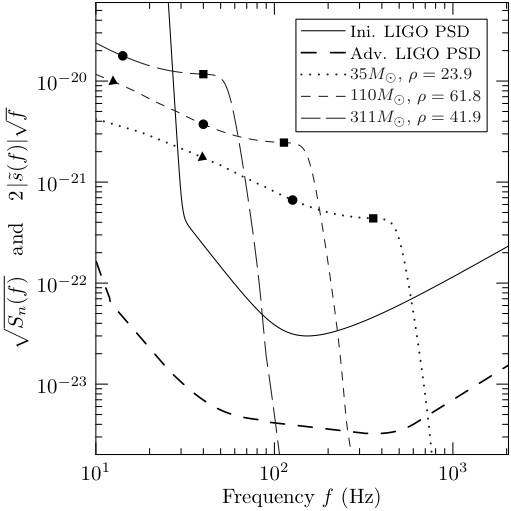
\includegraphics[width=\linewidth]{figures/ninja2/StildesAndInitialPSD}
  \caption[Hybrid MayaKranc waveform scaled to various total masses]{
  \label{fig:Ninja2StildesAndInitialPSD}
    The hybrid $q=2$, non-spinning MayaKranc waveform scaled to various total
    masses, with sources optimally oriented and placed at
    \unit[100]{Mpc}, shown against the Initial- and Advanced-LIGO
    noise curves.  Markers are placed along the lines at frequencies
    corresponding to various instantaneous frequencies of the
    waveforms.  The triangles represent the frequency at which the
    numeric waveform begins; the circle represents the ISCO frequency;
    and the square the light-ring.  The values given for $\rho$ use
    the Initial-LIGO noise curve.}
\end{figure}%

To address these issues NINJA-2 specifies the following minimal
requirements~\cite{ninja2-wiki}.  The raw numerical simulation should
include at least five orbits of usable data before merger (i.e., not
counting bursts of junk radiation or other significant noise).  Given
the computation cost of extending the NR waveforms, we instead require
stitching to a post-Newtonian inspiral approximant, which should be
performed at a GW frequency of $M\omega \leq 0.075$, where $M\omega$
is the frequency of the $(l = 2, m = \pm 2)$ harmonic. The full
waveform should be long enough to be entirely within the sensitivity
bands of LIGO and Virgo down to $10 \msun$ with a lower cutoff
frequency of 10 Hz, which corresponds to a starting GW frequency of
$M\omega = 0.003$.  The numerical-waveform (before any hybridization)
amplitude should be accurate to within 5\%, and the phase (as a
function of GW frequency) should have an accumulated uncertainty over
the entire inspiral, merger and ringdown, of no more than 0.5 radian.
The PN approximants used for hybridization should ideally use the
highest PN orders available, both in phase and amplitude.  These
minimal accuracy requirements are motivated by the results of the
Samurai project~\cite{Hannam:2009hh}, and studies performed in
preparation for the NR-AR collaboration project~\cite{ninja-wiki}.

The NINJA-2 project encourages although does not require the addition
of higher-order modes.  We chose to restrict attention to non-spinning
waveforms and waveforms with spins aligned or anti-aligned with the
orbital angular momentum.  There are sufficient open questions
regarding these restricted cases to make this analysis interesting,
without adding the additional complications on both the NR and data
analysis sides associated with precession. 

A total of 60 waveforms from 8 groups were contributed, these are
summarized in tables ~\ref{tab:ninja2_bam}, \ref{tab:ninja2_fau},
\ref{tab:ninja2_gatech}, \ref{tab:ninja2_lean},
\ref{tab:ninja2_llama}, \ref{tab:ninja2_rit}, \ref{tab:ninja2_spec},
\ref{tab:ninja2_uiuc} and a map of the parameter values is shown in
figure~\ref{f:ninja2_param_map}.

\begin{table}
\begin{center}
\begin{tabular}{|l|r|r|r|l|c|}
\hline
Run & $q$ & Spin1${}_z$ & Spin2${}_z$ & pN Approx. & Refs \\
\hline
BAM\_D10spp85\_80.T4.hyb.n2 & 1 & 0.85 & 0.85 & TaylorT4 & \cite{Hannam:2007wf,Brugmann:2008zz} \\
BAM\_D10spp85\_80.T1.hyb.n2 & 1 & 0.85 & 0.85 & TaylorT1 & \cite{Hannam:2007wf,Brugmann:2008zz} \\
BAM\_D125smm50Nep\_80.T1.hyb.n2 & 1 & -0.50 & -0.50 & TaylorT1 & \cite{Hannam:2007wf,Brugmann:2008zz} \\
BAM\_D125smm50Nep\_80.T4.hyb.n2 & 1 & -0.50 & -0.50 & TaylorT4 & \cite{Hannam:2007wf,Brugmann:2008zz} \\
BAM\_D13smm75Nep\_96.T4.hyb.n2 & 1 & -0.75 & -0.75 & TaylorT4 & \cite{Hannam:2007wf,Brugmann:2008zz} \\
BAM\_D13smm75Nep\_96.T1.hyb.n2 & 1 & -0.75 & -0.75 & TaylorT1 & \cite{Hannam:2007wf,Brugmann:2008zz} \\
BAM\_D13smm85Nep\_88.T4.hyb.n2 & 1 & -0.85 & -0.85 & TaylorT4 & \cite{Hannam:2007wf,Brugmann:2008zz} \\
BAM\_D13smm85Nep\_88.T1.hyb.n2 & 1 & -0.85 & -0.85 & TaylorT1 & \cite{Hannam:2007wf,Brugmann:2008zz} \\
BAM\_D11spp50\_96.T4.hyb.n2 & 1 & 0.50 & 0.50 & TaylorT4 & \cite{Hannam:2007wf,Brugmann:2008zz} \\
BAM\_D11spp50\_96.T1.hyb.n2 & 1 & 0.50 & 0.50 & TaylorT1 & \cite{Hannam:2007wf,Brugmann:2008zz} \\
BAM\_D10spp75\_80.T1.hyb.n2 & 1 & 0.75 & 0.75 & TaylorT1 & \cite{Hannam:2007wf,Brugmann:2008zz} \\
BAM\_D10spp75\_80.T4.hyb.n2 & 1 & 0.75 & 0.75 & TaylorT4 & \cite{Hannam:2007wf,Brugmann:2008zz} \\
BAM\_D12smm25Nep\_80.T4.hyb.n2 & 1 & -0.25 & -0.25 & TaylorT4 & \cite{Hannam:2007wf,Brugmann:2008zz} \\
BAM\_D12smm25Nep\_80.T1.hyb.n2 & 1 & -0.25 & -0.25 & TaylorT1 & \cite{Hannam:2007wf,Brugmann:2008zz} \\
BAM\_EP\_um4\_D10-n96.T4.hyb.n2 & 4 & 0.00 & 0.00 & TaylorT4 & \cite{Hannam:2007wf,Brugmann:2008zz} \\
BAM\_EP\_um4\_D10-n96.T1.hyb.n2 & 4 & 0.00 & 0.00 & TaylorT1 & \cite{Hannam:2007wf,Brugmann:2008zz} \\
BAM\_um3\_88.T4.hyb.n2 & 3 & 0.00 & 0.00 & TaylorT4 & \cite{Hannam:2007wf,Brugmann:2008zz} \\
BAM\_um3\_88.T1.hyb.n2 & 3 & 0.00 & 0.00 & TaylorT1 & \cite{Hannam:2007wf,Brugmann:2008zz} \\
BAM\_um2\_88.T1.hyb.n2 & 2 & 0.00 & 0.00 & TaylorT1 & \cite{Hannam:2007wf,Brugmann:2008zz} \\
BAM\_um2\_88.T4.hyb.n2 & 2 & 0.00 & 0.00 & TaylorT4 & \cite{Hannam:2007wf,Brugmann:2008zz} \\
BAM\_R6\_PN\_80.T1.hyb.n2 & 1 & 0.00 & 0.00 & TaylorT1 & \cite{Hannam:2007wf,Brugmann:2008zz} \\
BAM\_R6\_PN\_80.T4.hyb.n2 & 1 & 0.00 & 0.00 & TaylorT4 & \cite{Hannam:2007wf,Brugmann:2008zz} \\
BAM\_D12spp25\_96.T4.hyb.n2 & 1 & 0.25 & 0.25 & TaylorT4 & \cite{Hannam:2007wf,Brugmann:2008zz} \\
BAM\_D12spp25\_96.T1.hyb.n2 & 1 & 0.25 & 0.25 & TaylorT1 & \cite{Hannam:2007wf,Brugmann:2008zz} \\
BAM\_q2a0a025\_T\_96\_344.T1.hyb.n2.bbh & 2 & 0.25 & 0.00 & {} & \cite{,Brugmann:2008zz} \\
BAM\_q2a0a025\_T\_96\_344.T4.hyb.n2.bbh & 2 & 0.25 & 0.00 & {} & \cite{,Brugmann:2008zz} \\
\hline
\end{tabular}
\end{center}
\caption[BAM submissions to NINJA-2]{
\label{tab:ninja2_bam}
BAM submissions to NINJA-2}
\end{table}

\begin{table}
\begin{center}
\begin{tabular}{|l|r|r|r|l|c|}
\hline
Run & $q$ & Spin1${}_z$ & Spin2${}_z$ & pN Approx. & Refs \\
\hline
BAM\_hybrid\_om0.025etmq3S0.4- & 3 & 0.40 & 0.60 & TaylorT4 & \cite{none,???} \\
0\_0\_S0.6\_0\_0\_72 &  &  &  &  &  \\
\hline
\end{tabular}
\end{center}
\caption[FAU submissions to NINJA-2]{
\label{tab:ninja2_fau}
FAU submissions to NINJA-2}
\end{table}

\begin{table}
\begin{center}
\begin{tabular}{|l|r|r|r|l|c|}
\hline
Run & $q$ & Spin1${}_z$ & Spin2${}_z$ & pN Approx. & Refs \\
\hline
MayaKranc\_D12\_a0.00\_m129\_nj & 1 & 0.00 & 0.00 & TaylorT4 & \cite{,} \\
MayaKranc\_D10\_a0.90\_m129\_nj & 1 & 0.90 & 0.90 & TaylorT4 & \cite{,} \\
MayaKranc\_D10\_a0.20\_m77\_nj & 1 & 0.20 & 0.20 & TaylorT4 & \cite{,} \\
MayaKranc\_D10\_a0.60\_m77\_nj & 1 & 0.60 & 0.60 & TaylorT4 & \cite{,} \\
MayaKranc\_D12\_a0.60\_m103\_nj & 1 & 0.60 & 0.60 & TaylorT4 & \cite{,} \\
MayaKranc\_Sp02py0935th90\_gr & 1 & 0.80 & 0.00 & TaylorT4 & \cite{,} \\
MayaKranc\_D12\_a0.80\_m103\_nj & 1 & 0.80 & 0.80 & TaylorT4 & \cite{,} \\
MayaKranc\_D12\_a0.00\_q2\_m90\_nj & 2 & 0.00 & 0.00 & TaylorT4 & \cite{,} \\
MayaKranc\_D11\_a0.20\_q2\_m90\_nj & 2 & 0.02 & 0.09 & TaylorT4 & \cite{,} \\
MayaKranc\_D10\_a0.40\_m90\_nj & 1 & 0.40 & 0.40 & TaylorT4 & \cite{,} \\
MayaKranc\_D10\_a0.80\_m90\_nj & 1 & 0.80 & 0.80 & TaylorT4 & \cite{,} \\
MayaKranc\_D12\_a0.40\_m103\_nj & 1 & 0.40 & 0.40 & TaylorT4 & \cite{,} \\
MayaKranc\_D12\_a0.20\_m103\_nj & 1 & 0.20 & 0.20 & TaylorT4 & \cite{,} \\
\hline
\end{tabular}
\end{center}
\caption[GATech submissions to NINJA-2]{
\label{tab:ninja2_gatech}
GATech submissions to NINJA-2}
\end{table}

\begin{table}
\begin{center}
\begin{tabular}{|l|r|r|r|l|c|}
\hline
Run & $q$ & Spin1${}_z$ & Spin2${}_z$ & pN Approx. & Refs \\
\hline
dq4 & 4 & 0.00 & 0.00 & TaylorT1 & \cite{,Sperhake:2006cy} \\
\hline
\end{tabular}
\end{center}
\caption[LEAN submissions to NINJA-2]{
\label{tab:ninja2_lean}
LEAN submissions to NINJA-2}
\end{table}

\begin{table}
\begin{center}
\begin{tabular}{|l|r|r|r|l|c|}
\hline
Run & $q$ & Spin1${}_z$ & Spin2${}_z$ & pN Approx. & Refs \\
\hline
Llama\_d550-h64-Hybrid & 1 & 0.00 & 0.00 & 3.5pNTaylorF2 & \cite{Reisswig:2009rx,Reisswig:2009rx} \\
Llama\_d4d4-q1--D10-h64-r250.T4.hybrid & 1 & -0.40 & -0.40 & TaylorT4 & \cite{Pollney:2010hs,Pollney:2009yz,} \\
Llama\_d4d4-q1--D10-h64-r250.T1.hybrid & 1 & -0.40 & -0.40 & TaylorT1 & \cite{Pollney:2010hs,Pollney:2009yz,} \\
Llama\_u4u4-q1--D8-h64-r250.T1.hybrid & 1 & 0.40 & 0.40 & TaylorT1 & \cite{Pollney:2010hs,Pollney:2009yz,} \\
Llama\_u4u4-q1--D8-h64-r250.T4.hybrid & 1 & 0.40 & 0.40 & TaylorT4 & \cite{Pollney:2010hs,Pollney:2009yz,} \\
Llama\_d5q2-h016-Hybrid & 2 & 0.00 & 0.00 & 3.5pNTaylorF2 & \cite{,Reisswig:2009rx} \\
Llama\_u2u2-q1--D8-h64-r250.T1.hybrid & 1 & 0.20 & 0.20 & TaylorT1 & \cite{Pollney:2010hs,Pollney:2009yz,} \\
Llama\_u2u2-q1--D8-h64-r250.T4.hybrid & 1 & 0.20 & 0.20 & TaylorT4 & \cite{Pollney:2010hs,Pollney:2009yz,} \\
Llama\_d2d2-q1--D10-h64-r250.T1.hybrid & 1 & -0.20 & -0.20 & TaylorT1 & \cite{Pollney:2010hs,Pollney:2009yz,} \\
Llama\_d2d2-q1--D10-h64-r250.T4.hybrid & 1 & -0.20 & -0.20 & TaylorT4 & \cite{Pollney:2010hs,Pollney:2009yz,} \\
\hline
\end{tabular}
\end{center}
\caption[Llama submissions to NINJA-2]{
\label{tab:ninja2_llama}
Llama submissions to NINJA-2}
\end{table}

\begin{table}
\begin{center}
\begin{tabular}{|l|r|r|r|l|c|}
\hline
Run & $q$ & Spin1${}_z$ & Spin2${}_z$ & pN Approx. & Refs \\
\hline
LazEV\_D8.4\_10to1\_nj\_hybrid & 10 & 0.00 & 0.00 & TaylorT4 & \cite{Campanelli:2005dd} \\
\hline
\end{tabular}
\end{center}
\caption[RIT submissions to NINJA-2]{
\label{tab:ninja2_rit}
RIT submissions to NINJA-2}
\end{table}

\begin{table}
\begin{center}
\begin{tabular}{|l|r|r|r|l|c|}
\hline
Run & $q$ & Spin1${}_z$ & Spin2${}_z$ & pN Approx. & Refs \\
\hline
SpEC\_q6s0 & 6 & 0.00 & 0.00 & TaylorT1 & \cite{SpECWebsite} \\
SpEC\_q4s0 & 4 & 0.00 & 0.00 & TaylorT2 & \cite{SpECWebsite} \\
SpEC\_EqualMassAntiAlignedSpins & 1 & -0.44 & -0.44 & NA & \cite{chu-2009,SpECWebsite} \\
SpEC\_q1s-0.95 & 1 & -0.95 & -0.95 & TaylorT1 & \cite{SpECWebsite} \\
SpEC\_q2s0 & 2 & 0.00 & 0.00 & TaylorT2 & \cite{SpECWebsite} \\
SpEC\_EqualMassAlignedSpins & 1 & 0.44 & 0.44 & NA & \cite{chu-2009,SpECWebsite} \\
SpEC\_q3s0 & 3 & 0.00 & 0.00 & TaylorT2 & \cite{SpECWebsite} \\
SpEC\_EqualMassNonspinning & 1 & 0.00 & 0.00 & TaylorT4 & \cite{Scheel:2008rj,SpECWebsite} \\
\hline
\end{tabular}
\end{center}
\caption[SpEC submissions to NINJA-2]{
\label{tab:ninja2_spec}
SpEC submissions to NINJA-2}
\end{table}

\begin{table}
\begin{center}
\begin{tabular}{|l|r|r|r|l|c|}
\hline
Run & $q$ & Spin1${}_z$ & Spin2${}_z$ & pN Approx. & Refs \\
\hline
UIUC\_spin\_-0.25\_om0.0528\_22-HYBRID & 1 & -0.25 & -0.25 & NA & \cite{none} \\
UIUC\_spin\_0.85\_om0.0536\_22-HYBRID & 1 & 0.85 & 0.85 & NA & \cite{none} \\
\hline
\end{tabular}
\end{center}
\caption[UIUC submissions to NINJA-2]{
\label{tab:ninja2_uiuc}
UIUC submissions to NINJA-2}
\end{table}


\begin{figure}
  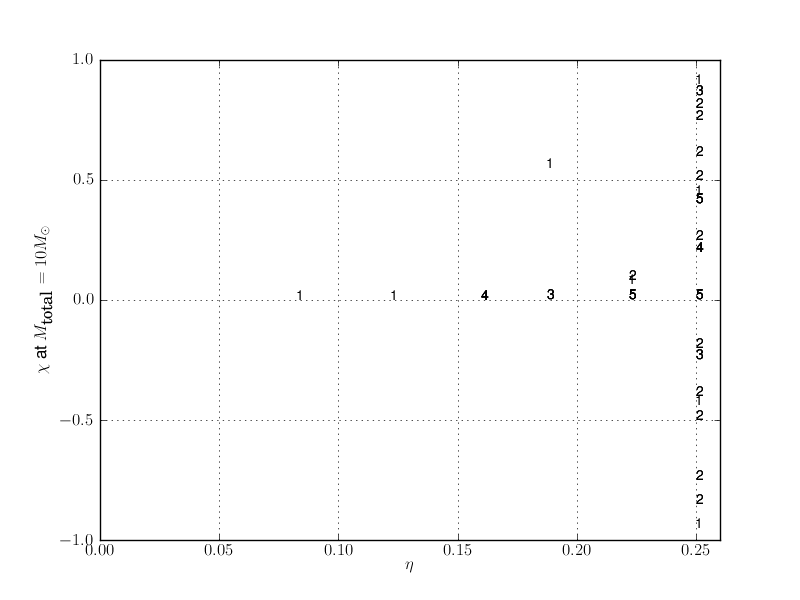
\includegraphics[width=\linewidth]{figures/ninja2/ninja2_cat.png}
  \caption[Parameters of the NINJA-2 submissions]{
  \label{f:ninja2_param_map}
Parameters of the NINJA-2 hybrid waveform submissions showing the
symmetric mass ratio $\eta=m_1 m_2 /(m_1+m_2)^2$ and dimensionless
spin parameter $\chi=(S_1/m_1 + S_2/m_2)/(m_1+m_2)$ after scaling the
waveforms to a reference total mass of 10 $\msun$.  The numbers indicate 
how many distinct waveforms with the specified parameters were submitted.}
\end{figure}%

\section{Verifying the hybrid waveforms}

Each NR group verified that their waveforms met the minimum NINJA-2
requirements before submission.  Once submitted, a series of checks
were performed in order to validate the waveforms against each other.

In the first stage the post-Newtonian expressions and codes were
compared against each other and the literature.  This required several
iterations, but resulted in a set of codes in various languages that
produce waveforms that all agree in both phase and amplitude. 

\subsection{Time-domain and frequency-domain checks}

In the second stage the complete hybrid waveforms were examined.
We first plotted the last 40 cycles of each waveform -- enough to
include the full NR portion, the hybridization region, and some of the
pN portion -- and looked for any anomalies such as those present in
some of the NINJA-1 waveforms in figure~\ref{fig:NR-Reh22}.

\iffalse
  A few such
features were indeed visible, spotting them in this way allowed them
to be corrected.  One example is shown in figure (\Note{show the dq4
waveform before and after, note this was due to a problem integrating
psi4, and discuss this stage a little in the NR section of chapter
3}).
\fi

The amplitudes of the Fourier transform of the complete waveforms were
also plotted.  This analysis revealed unphysical features, primarily
due to hybridization.  An example is shown in
figure~\ref{f:ninja2_freq_hybrids}, which shows a visible ``kink'' in
the waveform at the hybridization frequency.  This feature is no
longer present in the waveform after the hybrid was reconstructed.

\begin{figure}
  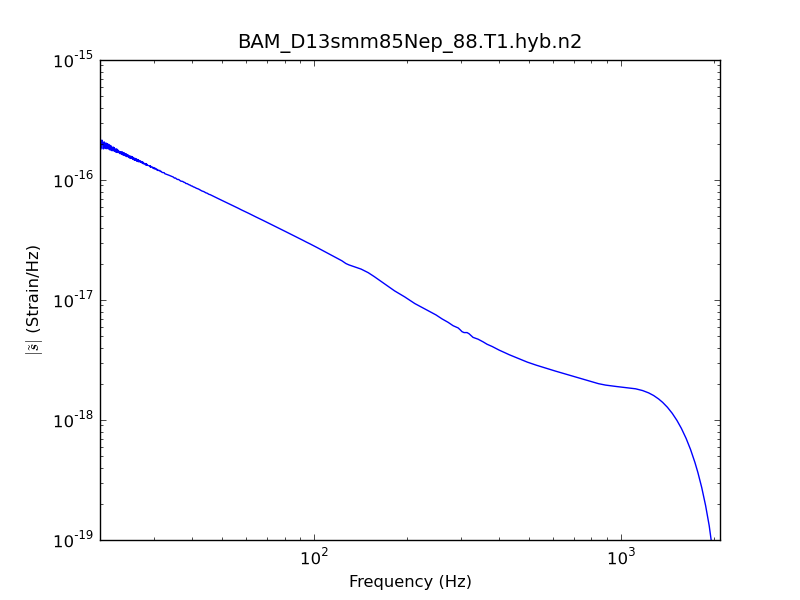
\includegraphics[width=0.5\linewidth]{figures/ninja2/BAM_D13smm85Nep_88_T1_hyb_n2_amp_old}
  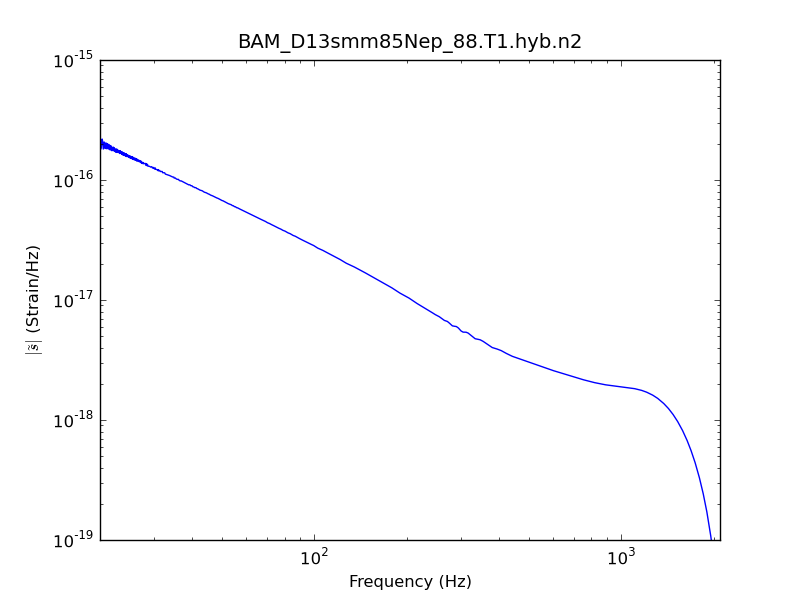
\includegraphics[width=0.5\linewidth]{figures/ninja2/BAM_D13smm85Nep_88_T1_hyb_n2_amp_new} \\
  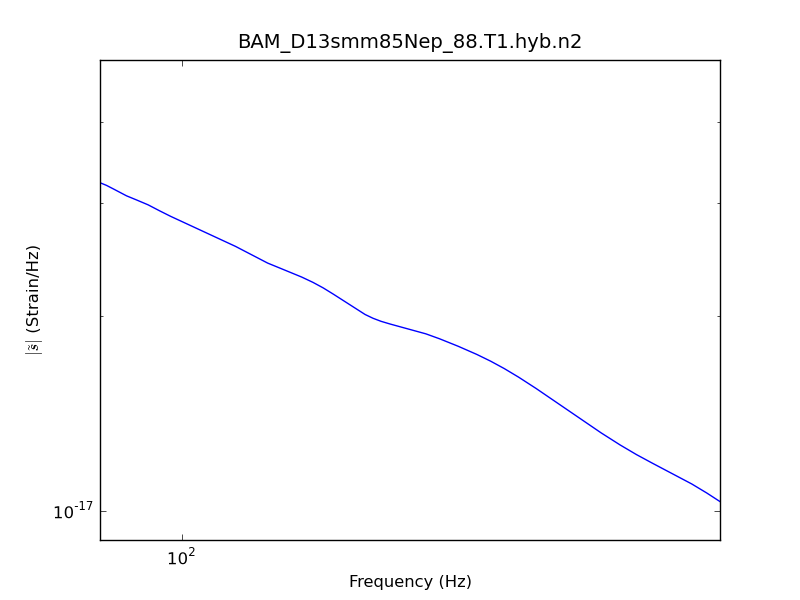
\includegraphics[width=0.5\linewidth]{figures/ninja2/BAM_D13smm85Nep_88_T1_hyb_n2_amp_old_zoom}
  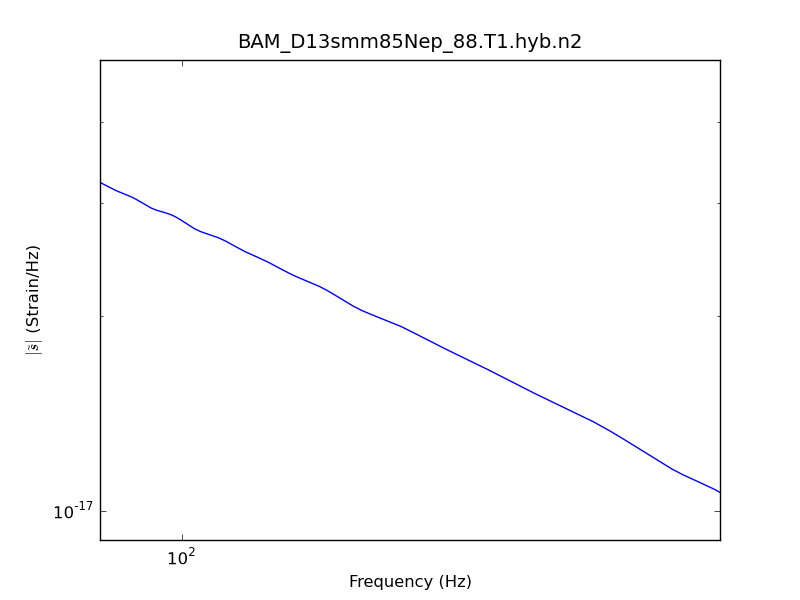
\includegraphics[width=0.5\linewidth]{figures/ninja2/BAM_D13smm85Nep_88_T1_hyb_n2_amp_new_zoom} \\
  \caption[Frequency-domain hybrid NINJA-2 waveforms]{
  \label{f:ninja2_freq_hybrids}
Fourier amplitude of the (2,2) mode of a sample NINJA-2 hybrid
waveform from the BAM/AEI group.  The waveform has been scaled to 10
$\msun$ and placed 1 Mpc from the detector to give it physical units.
The waveform on the top left is the version initially submitted, note
there is a small visible ``kink'' in the waveform at around 100 Hz.
The waveform on the top right has been re-hybridized and
there is no longer a visible kink.  On the bottom, the same waveform
before and after rehybridization, zoomed into the region in question.
This feature did not show up in the time domain view of the waveform.}
\end{figure}%


\subsection{Overlap comparisons}
\label{ssec:ninja2_overlap_comparisons}

In this check the waveforms were compared against each other using
standard data-analysis techniques, in particular the overlap defined
in equation~\ref{eq:OverlapDefinition}  using the initial LIGO noise
curve.  The waveforms were grouped into sets with identical
parameters.  For each set one waveform was chosen as the reference and
the overlap with all the other waveforms was calculated over a range of
masses, optimizing over the unknown coalescence time and phase as
usual.  This process was then repeated, taking each of the other
waveforms as the reference in turn.

There is an important subtlety involved in calculating these overlaps.
Recall from section~\ref{sec:ihope_match_filter} that the output of
the matched filter is a time series from which the point with the
largest value is chosen in order to maximize over time.  When
comparing two very similar waveforms, such as two numeric simulations
of the same system, the overlap function becomes very sharply peaked.
It is therefore imperative that the sample rate used in calculating 
the overlap be large enough to find the true maximum.

This issue is demonstrated in figure~\ref{f:overlap_sample_frequency}.
This figure shows the overlap function resulting from the comparison
of two equal-mass, non-spinning waveforms sampled at four different
rates.  At 40906 Hz, the sample rate used within the LIGO pipeline,
the peak of the function is missed and the overlap is underestimated.
The consequence of this is illustrated in
figure~\ref{f:overlap_wiggles} which shows that the overlap as a
function of mass exhibits oscillations.  The mass determines the length
of the waveform, as this length changes the waveforms slide with
respect to the grid of sample points, and the overlap function traces
out this beating.  Consequently, all overlaps in this chapter were
calculated at 32768 Hz.

\begin{figure}
  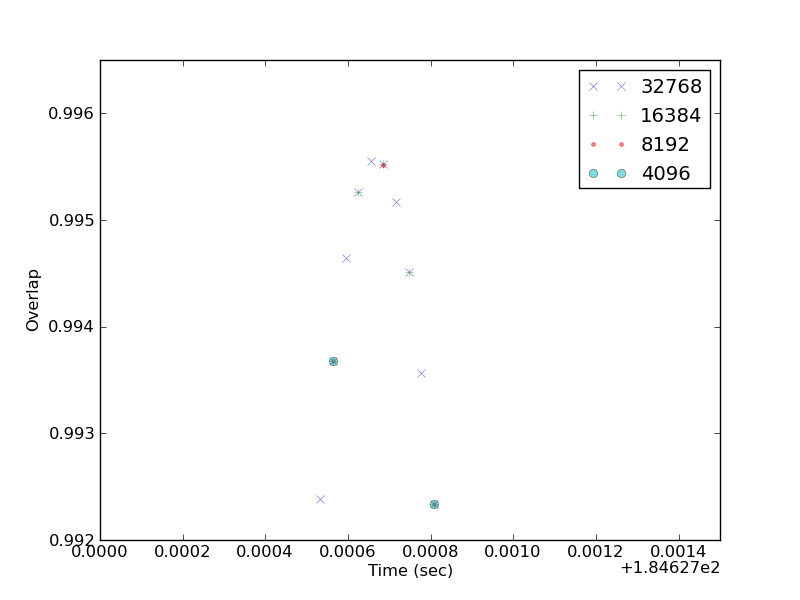
\includegraphics[width=\linewidth]{figures/ninja2/overlap_time_series}
  \caption[Sensitivity of the overlaps to sample rate]{
  \label{f:overlap_sample_frequency}
The overlap time series between the Georgia Tech and SpEC equal-mass,
non-spinning waveforms at different sample rates.  At 4096 Hz the
sample point nearest the maximum is sufficiently far that the overlap
is underestimated to an extent which is significant in doing such
comparisons, where we are interested in differences to one part in
$10^{-5}$.
}
\end{figure}%


\begin{figure}
  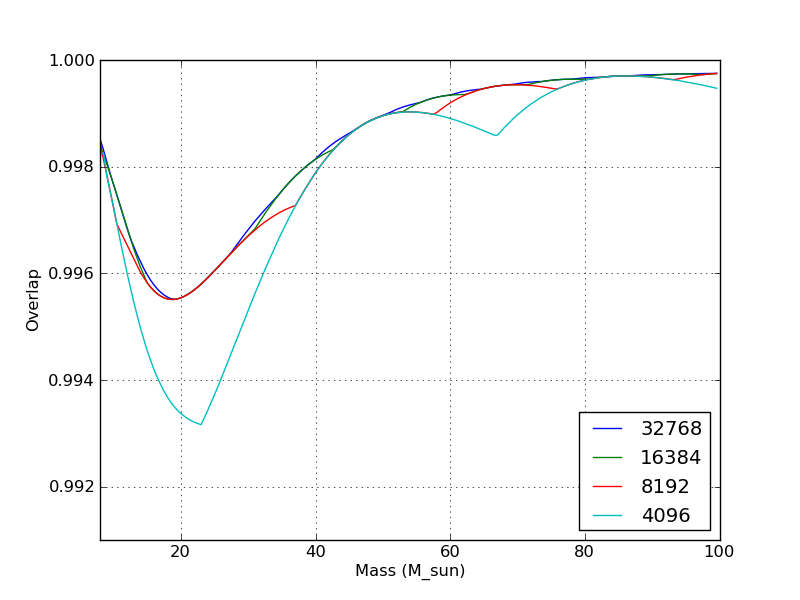
\includegraphics[width=\linewidth]{figures/ninja2/resolutions}
  \caption[Consequence of undersampling the overlap function]{
  \label{f:overlap_wiggles}
Overlaps between the Georgia Tech and SpEC equal-mass, non-spinning
waveforms, as a function of mass, at different sample rates.  At 4096
Hz the Consequence of undersampling the overlap function.  As the
waveform lengths change with mass they beat against the griding caused
by discrete sampling.  This produces periodic beats, most evident in
the overlaps sampled at 4096 Hz.}
\end{figure}%

For reference we first present comparisons between time-domain
post-Newtonian waveforms of the kind used to construct hybrid
waveforms.  These are shown in figure~\ref{f:pn_overlaps}.  Overlaps
between hybrid waveforms constructed using different pN approximants
will not agree better than the values presented here at low mass,
where the pN portion of the waveform extends through the most
sensitive portion of the LIGO band.


\begin{figure}
  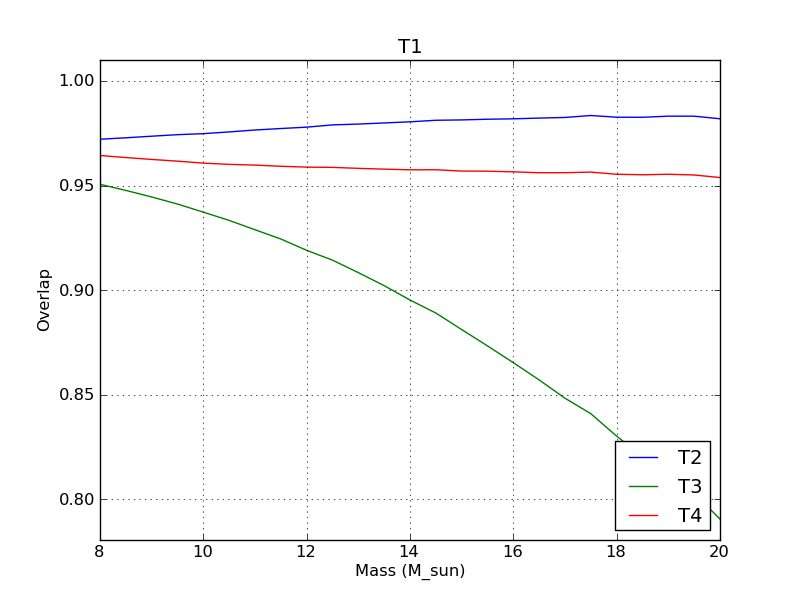
\includegraphics[width=\linewidth]{figures/ninja2/pn_figure03}
  \caption[Overlaps between pN waveforms as a function of mass]{
  \label{f:pn_overlaps}
Overlaps between equal-mass, non-spinning, post-Newtonian time-domain 
waveforms.  Note in particular the discrepancy between T1 and T4, as
these were used in the majority of the hybrid waveforms.
}
\end{figure}%

A sample set of overlaps, comparing all equal-mass, non-spinning
waveforms submissions is shown in figure~\ref{f:ninja2_overlap_test}.

At the high-mass end, where the numeric portion of the waveform
dominates the overlap, the overlaps approach 1.  This is as expected,
since all these waveforms model the same physical system.  This result
is nonetheless important, however, as the waveforms were produced with
different codes.

At the low-mass end, where the overlap is dominated by the
post-Newtonian portions of the waveform, the behavior is qualitatively
as expected from figure~\ref{f:pn_overlaps}.  Although some of the
overlaps, such as between the SpEC and BAM T1 waveforms, are notably
lower than would be expected based on pN considerations alone.  

In the region of $\approx 20 \msun$ all the overlaps drop, some more
significantly than others.  This is the region where the hybridization
is passing through the sensitive band.  The goal of
hybridization is to smoothly interpolate between the pN and NR
waveforms, and in cases where the pN and NR separately agree we would
expect this agreement to extend through the hybridization region.  We
see here, however, that this is not the case.  Different choices of
hybridization methods and parameters, as well as the frequencies over
which the hybridization is performed, can lead to waveforms with
significant mismatches.  

These initial results prompted a number of the NR groups to revise
their hybridization procedures, after which the overlaps were more in
line with the expected values.  The overlap plot produced with the
updated waveforms is shown along with the initial results in
figure~\ref{f:ninja2_overlap_test}.  It is worth noting that even
after rehybridizing there are still mismatches.  In particular, the
SpEC and MayaKranc submissions use the same hybridization method, the
same pN approximant and are simulating the same physical system.  The
only differences are the length of the NR waveforms and the
frequencies at which the hybridization is performed.  The question of
how many NR cycles are needed in order to produce a robust hybrid
waveform is an area of active research~\cite{MacDonald:2011}. 

\begin{figure}
  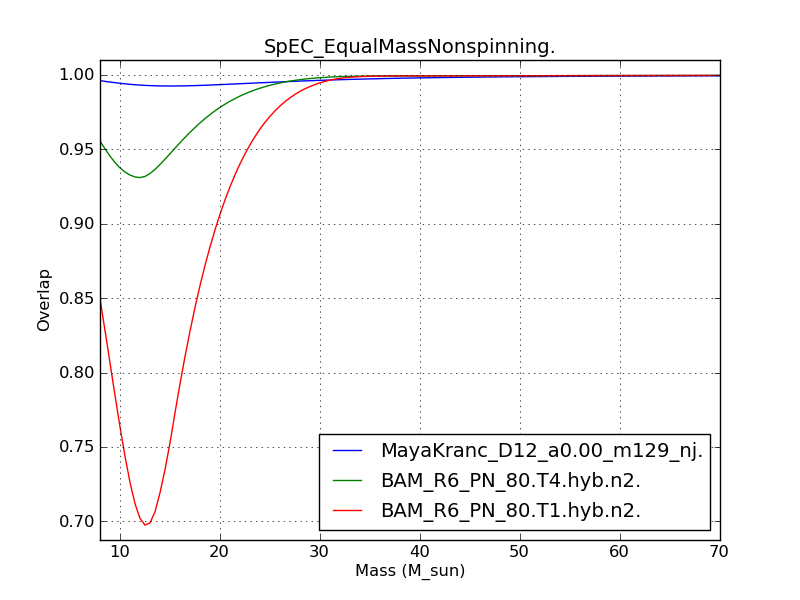
\includegraphics[width=0.5\linewidth]{figures/ninja2/q_1_z_0_figure03}
  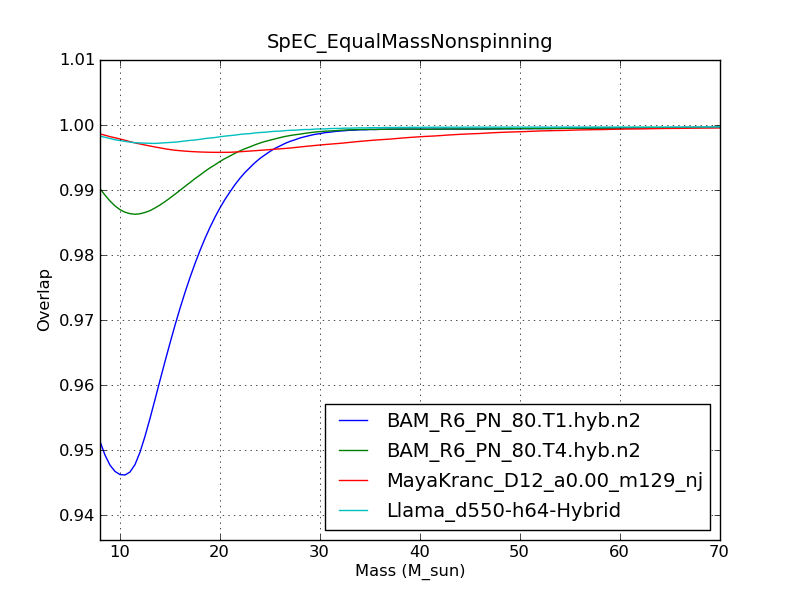
\includegraphics[width=0.5\linewidth]{figures/ninja2/figure2_1_0_16}
  \caption[Overlaps between NINJA-2 submissions maximized over time
and phase]{
  \label{f:ninja2_overlap_test}
Overlaps between the equal-mass, non-spinning NINJA-2 contributions,
maximized over time and phase.   For the original submissions (left)
overlaps are as low as 0.70 between waveforms using different pN
approximants and 0.94 for waveforms using the same approximant.  After
rehybridization (right) the waveforms achieve much higher overlaps,
with minima above 0.94 for different approximants and above 0.98 for
identical approximants.  The residual differences between waveforms
using TaylorT4 are due to hybridization details.  The Llama waveform
was accidentally omitted from the original runs.}
\end{figure}%

The full set of comparisons between the final versions of the
submissions appears at the end of the chapter, in figures
\ref{f:figure_1_-0d5} through \ref{f:figure_1_0d85}.

The overlap plots discussed thus far address the ``detection
question.''  By validating the waveforms against each other we ensure
that they are all capture the underlying physics well enough to
provide high overlaps with existing templates, which in turn implies
that these waveforms can be found in searches.  

We also extended these overlap studies by maximizing over the mass of
one of the waveforms, as well as the time and phase.  This addresses
the ``parameter estimation question,'' the bias in the recovered mass
gives an estimate of the minimum error that can be expected in
parameter estimation pipelines.  Example plots using the equal-mass,
non-spinning MayaKranc waveform as the signal and BAM plus two
different approximants as the template are shown in
figure~\ref{f:ninja2_max_over_mass_bam}.


\begin{figure}
  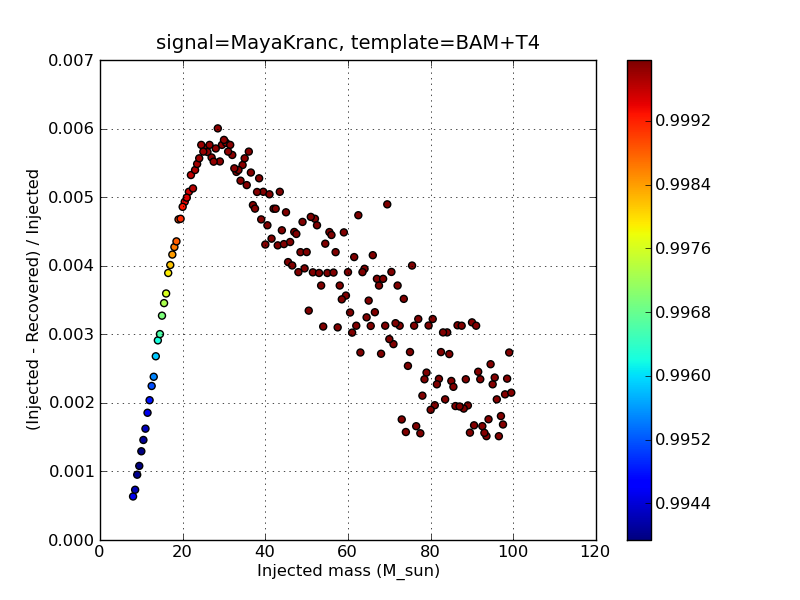
\includegraphics[width=0.5\linewidth]{figures/ninja2/maya_bamt4_max_over_m}
  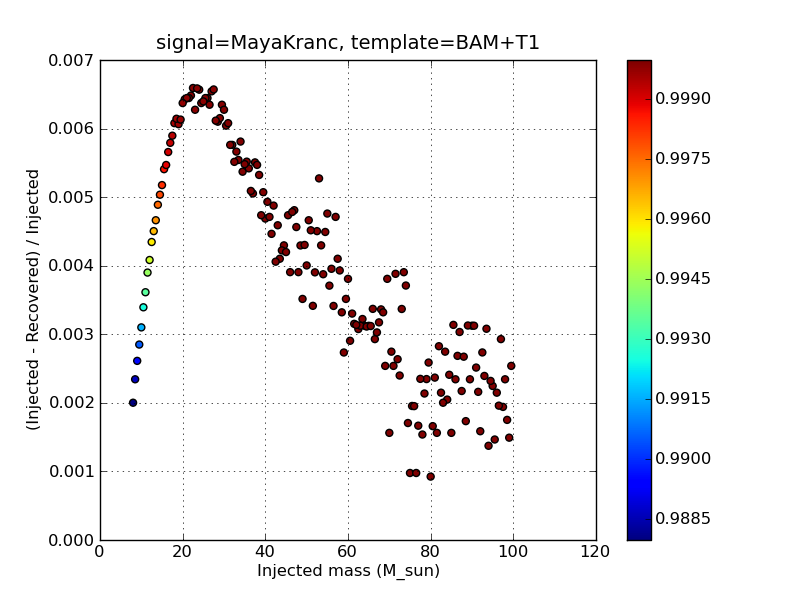
\includegraphics[width=0.5\linewidth]{figures/ninja2/maya_bamt1_max_over_m}
  \caption[Overlaps between NINJA-2 submissions maximized over mass]{
  \label{f:ninja2_max_over_mass_bam}
Overlaps (indicated by color) between the equal-mass, non-spinning
MayaKranc waveform taken as the signal, and the equal-mass,
non-spinning BAM waveform hybridized with TaylorT4 (left) and TaylorT1
(right) taken as templates.  Maximization is done over the mass of the
template, as well as over time and phase.  The x-axis gives the mass
of the signal, the y-axis gives the fractional difference between the
injected mass and the mass of the template that maximizes the overlap
Note the lower overall overlaps and mass bias at the low-mass end of
the figure on the right, where the two different pN waveforms dominate
the overlap.}
\end{figure}%

At the high-mass end the overlap is dominated by NR data, and as in
figure~\ref{f:ninja2_overlap_test} the overlaps are high without
needing to move off the signal mass.  At the low-mass end the same
result would be expected in a pure pN/pN comparison although there
is enough of the hybridization in-band to reduce the overlaps.  However,
changing the mass introduces a phase difference that accumulates over
all the cycles in-band, and so higher overlaps can not be achieved.
The result is optimal mass values close to the correct mass value, but
with a low overlap.

In the middle region these factors compete.  At higher masses the
overlap is reduced less by changing the mass and so the recovered
value can stray further from the injected value.  However as the
hybridization passes out of band this adjustment is no longer needed.

The same general behavior can be seen in comparisons between 
non-spinning, unequal-mass ($q=2$) waveforms, shown in
figure~\ref{f:max_over_m_q2}.  However, the overlaps drop slightly 
above $\approx 60 \msun$, suggesting a disagreement in the NR portion
of the waveforms.

The comparison between two equal-mass, spinning ($s_{1z} = s_{2z} =
0.4$) waveforms is shown in figure~\ref{f:max_over_m_z4}.  Here there
is a bias in recovered mass at the high-mass end, although the
overlaps are high.  This could suggest a problem with the overall
scaling of one of the waveforms, but more study is needed.


\begin{figure}
  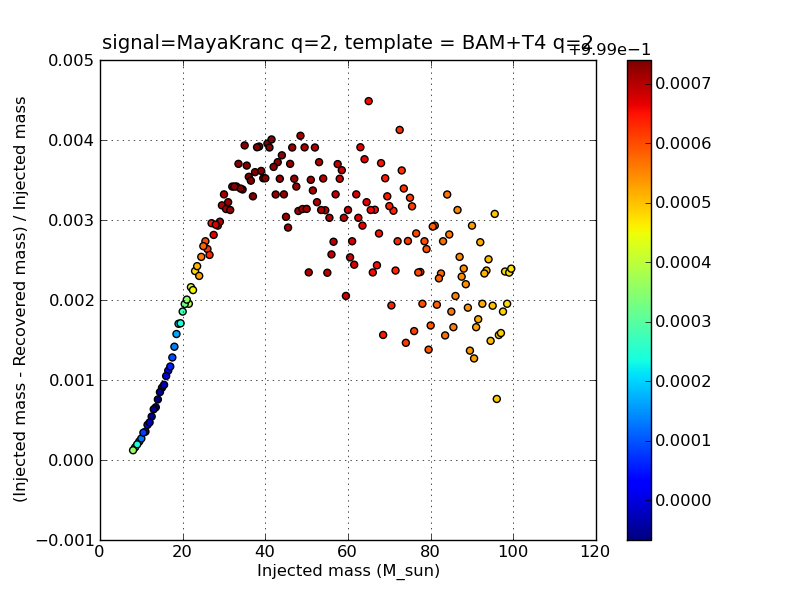
\includegraphics[width=\linewidth]{figures/ninja2/maya_bam_q2_max_over_m} 
  \caption[Overlaps between unequal-mass submissions maximized over mass]{
  \label{f:max_over_m_q2}
Overlaps (indicated by color) between the $q=2$ non-spinning MayaKranc
waveform taken as the signal, and the $q=2$, non-spinning BAM waveform
hybridized with TaylorT4 taken as the templates.  Maximization is done
over the mass of the template, as well as over time and phase.  The
x-axis gives the mass of the signal, the y-axis gives the fractional
difference between the injected mass and the mass of the template that
maximizes the overlap.  The low overlaps above $60 \msun$ may be due
to differences in the NR waveforms.}
\end{figure}%



\begin{figure}
  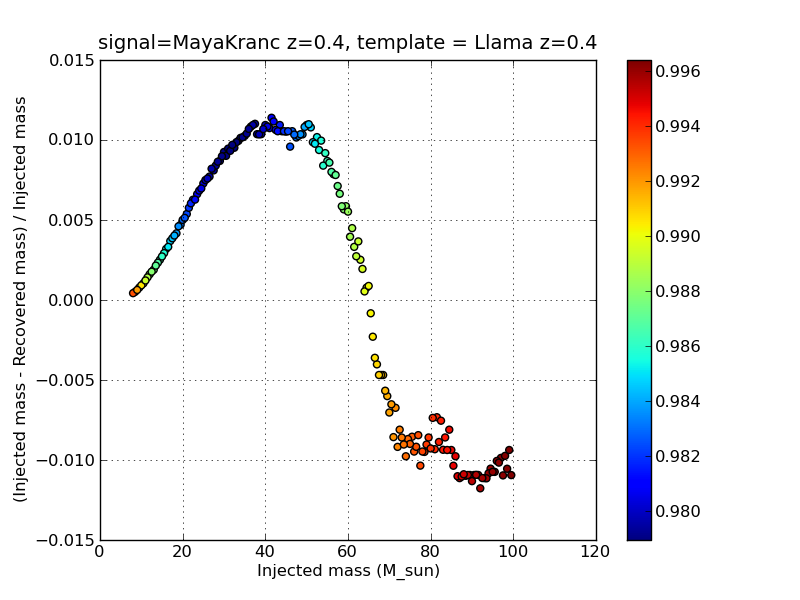
\includegraphics[width=\linewidth]{figures/ninja2/maya_llama_z0d4_max_over_m}
  \caption[Overlaps between spinning submissions maximized over mass]{
  \label{f:max_over_m_z4}
Overlaps (indicated by color) between the equal-mass $s_{1z} = s_{2z}
= 0.4$ MayaKranc waveform taken as the signal, and the equal-mass
$s_{1z} = s_{2z} = 0.4$ Llama waveform taken
as the template.  Maximization is done over the mass of the template,
as well as over time and phase.  The x-axis gives the mass of the
signal, the y-axis gives the fractional difference between the
injected mass and the mass of the template that maximizes the overlap.
The low overlaps above $60 \msun$ may be due to differences in the NR
waveforms.  The reason for the systematic bias at the high-mass end is
not clear.}
\end{figure}%


\section{Conclusion}

We have reviewed the hybrid waveforms submitted to the second NINJA
project.  Although many groups have contributed many waveforms, these
primarily cover only two lines  in the (mass ratio, $\chi$) plane,
leaving large regions of parameter space unexplored.  We also do not
consider precessing signals, which adds several dimensions to
parameter space.  These issues will be further explored in NINJA-3.

A major feature of NINJA-2, not present in NINJA-1, is the validation 
and comparisons of the submissions discussed in this chapter.  These 
efforts lead to dramatic improvements in the quality of the waveforms,
which in turn will enable data analysts to draw more quantitative 
conclusions on the behavior of their pipelines with respect to the
underlying physics.

There is evidence that hybridization choices and methods effect both
overlaps and parameter estimation.   The degree to which these effects
will bias searches is a question we hope NINJA-2 will be able to
answer.

In the next chapter we discuss the construction of data sets using
these waveforms, and present preliminary results from the CBC low-
high-mass pipelines.


%%%%%%%%%%%%%%%%
\clearpage

\iffalse
\begin{figure}
  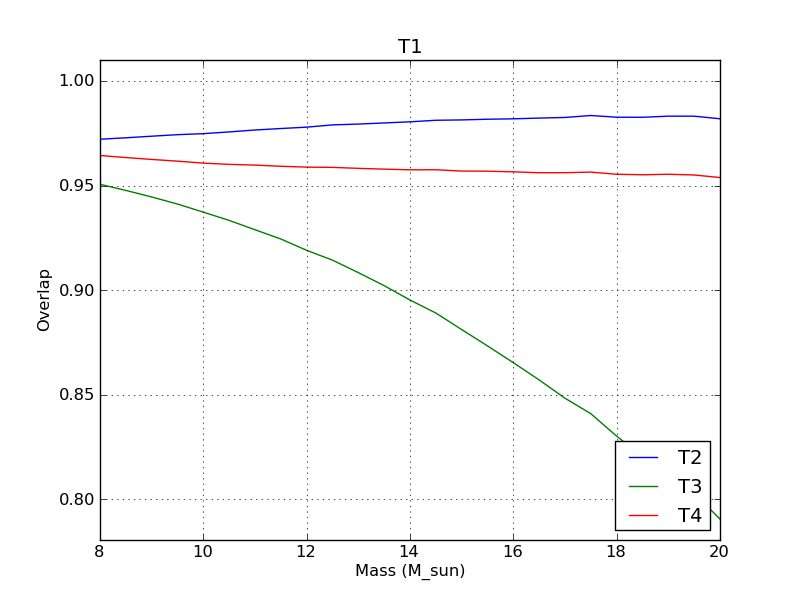
\includegraphics[width=0.5\linewidth]{figures/ninja2/pn_figure03.png} 
  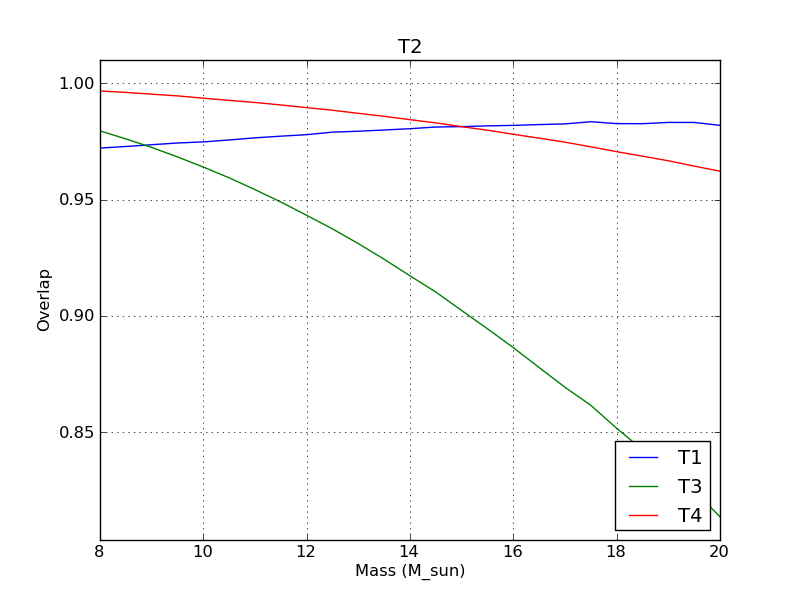
\includegraphics[width=0.5\linewidth]{figures/ninja2/pn_figure06.png} \\
  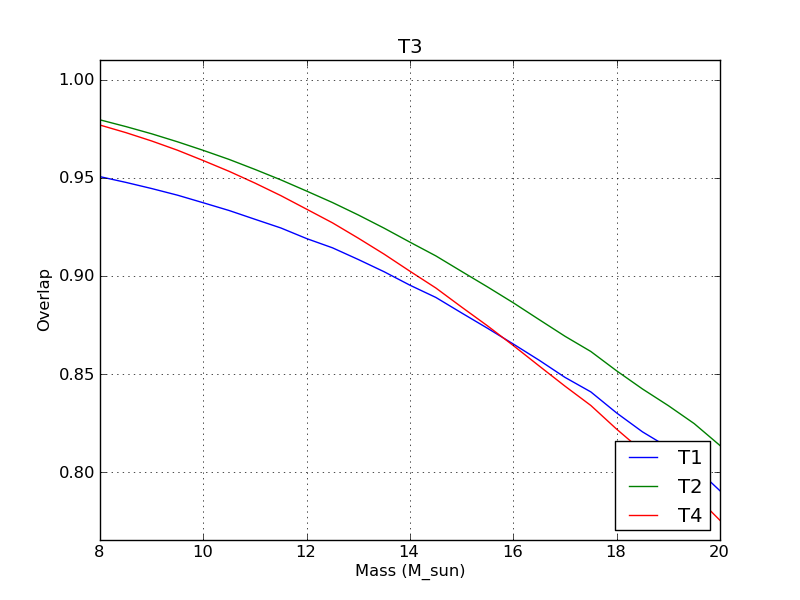
\includegraphics[width=0.5\linewidth]{figures/ninja2/pn_figure09.png} 
  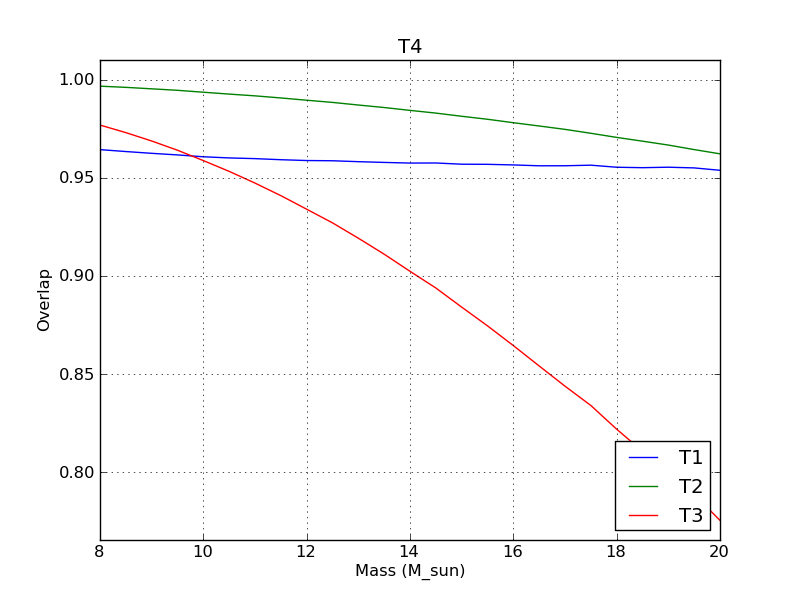
\includegraphics[width=0.5\linewidth]{figures/ninja2/pn_figure12.png} \\
  \caption[Overlap of time-domain pN waveforms, $q=1$ $S_{z1} = S_{z2} = 0$]{
  \label{f:figure_pn}
Overlap of time-domain pN waveforms, $q=1$ $S_{z1} = S_{z2} = 0$}
\end{figure}%
\fi

\begin{figure}
  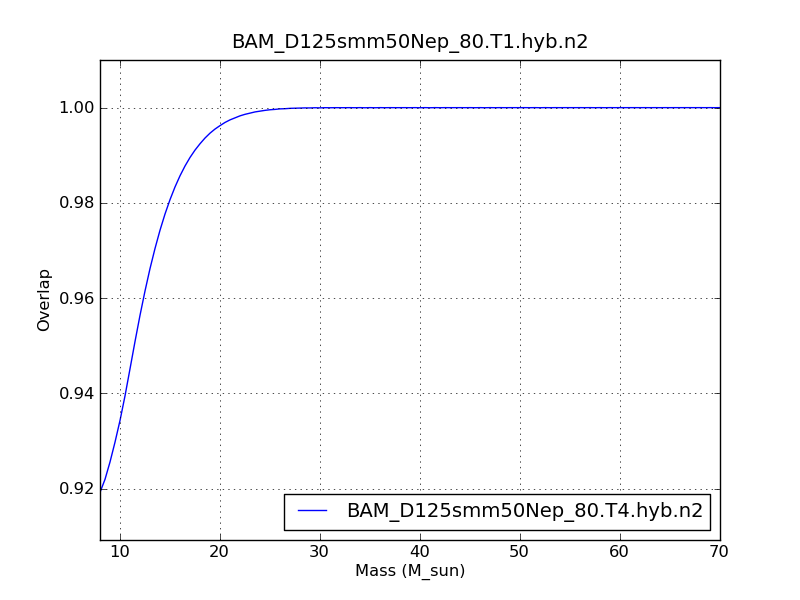
\includegraphics[width=\linewidth]{figures/ninja2/figure_1_-0d5_01.png}
  \caption[Overlap plots for $q=1$ $S_{z1} = S_{z2} = -0.5$]{
  \label{f:figure_1_-0d5}
Overlap plots for $q=1$ $S_{z1} = S_{z2} = -0.5$}
\end{figure}%


\begin{figure}
  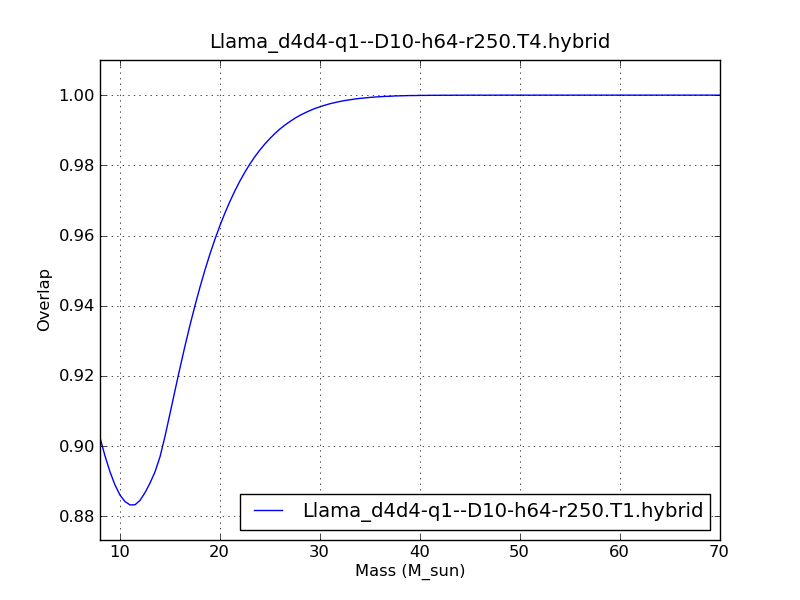
\includegraphics[width=\linewidth]{figures/ninja2/figure_1_-0d4_01.png}
  \caption[Overlap plots for $q=1$ $S_{z1} = S_{z2} = -0.4$]{
  \label{f:figure_1_-0d4}
Overlap plots for $q=1$ $S_{z1} = S_{z2} = -0.4$}
\end{figure}%


\begin{figure}
  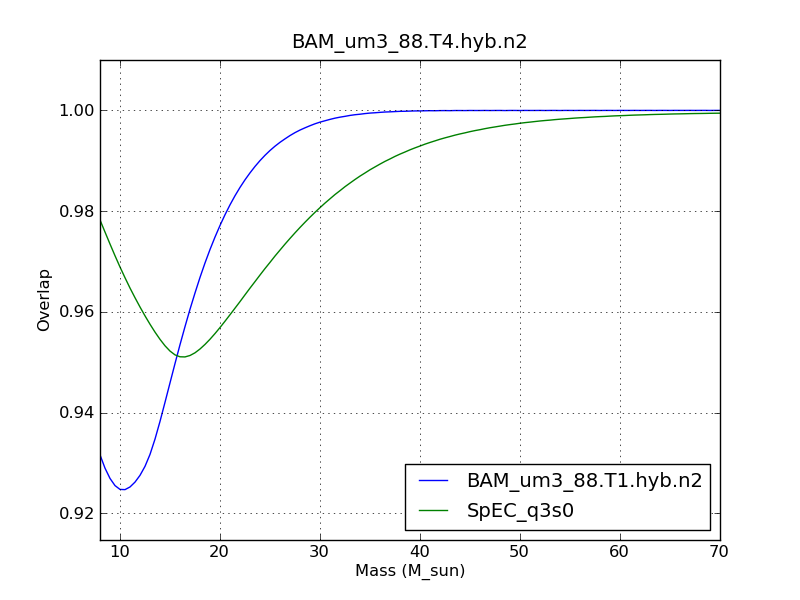
\includegraphics[width=0.5\linewidth]{figures/ninja2/figure_3_0_02.png} 
  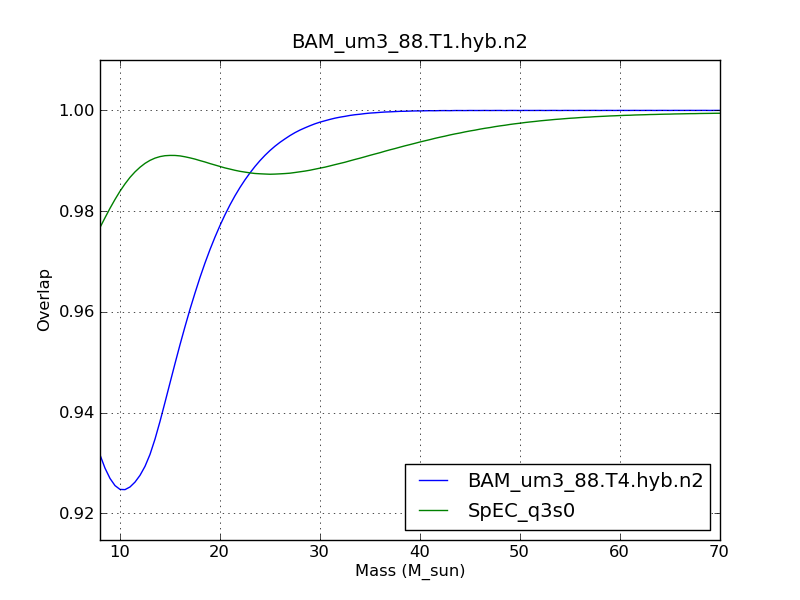
\includegraphics[width=0.5\linewidth]{figures/ninja2/figure_3_0_04.png} \\
  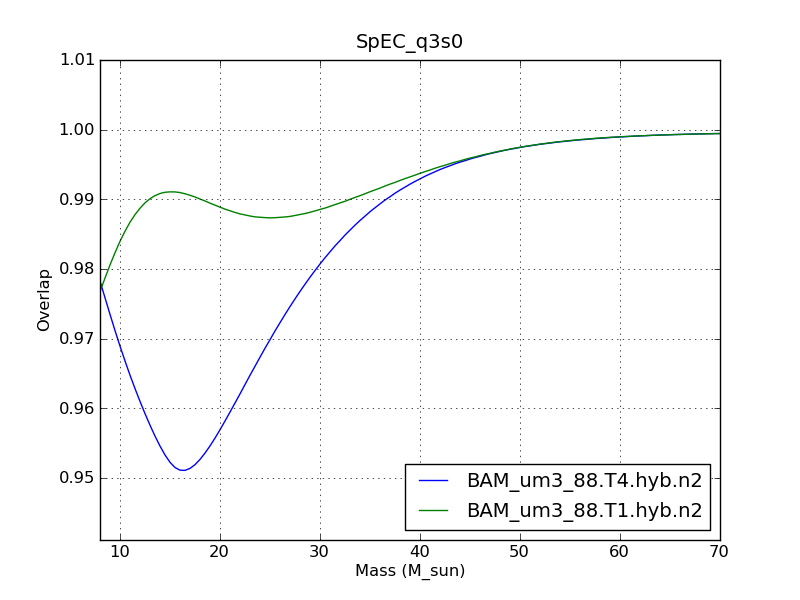
\includegraphics[width=0.5\linewidth]{figures/ninja2/figure_3_0_06.png} 
  \caption[Overlap plots for $q=3$ $S_{z1} = S_{z2} = 0$]{
  \label{f:figure_3_0}
Overlap plots for $q=3$ $S_{z1} = S_{z2} = 0$}
\end{figure}%


\begin{figure}
  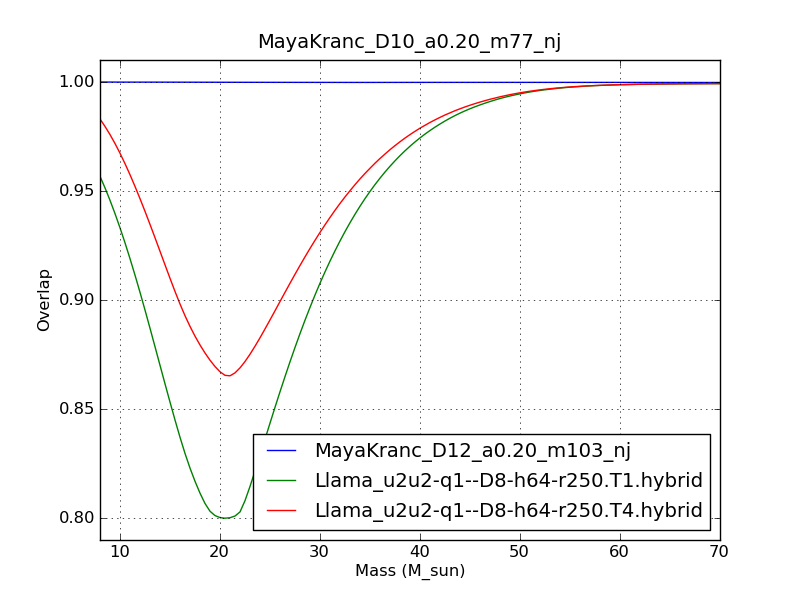
\includegraphics[width=0.5\linewidth]{figures/ninja2/figure_1_0d2_03.png} 
  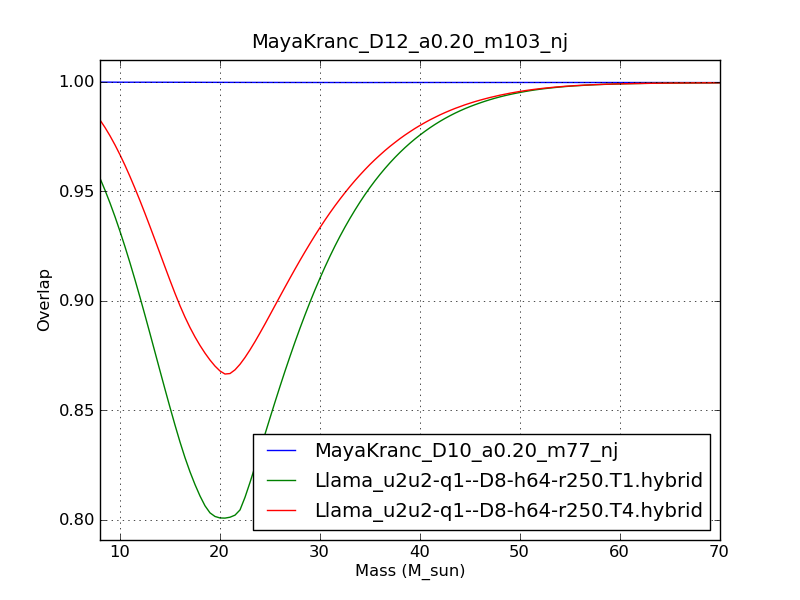
\includegraphics[width=0.5\linewidth]{figures/ninja2/figure_1_0d2_06.png} \\
  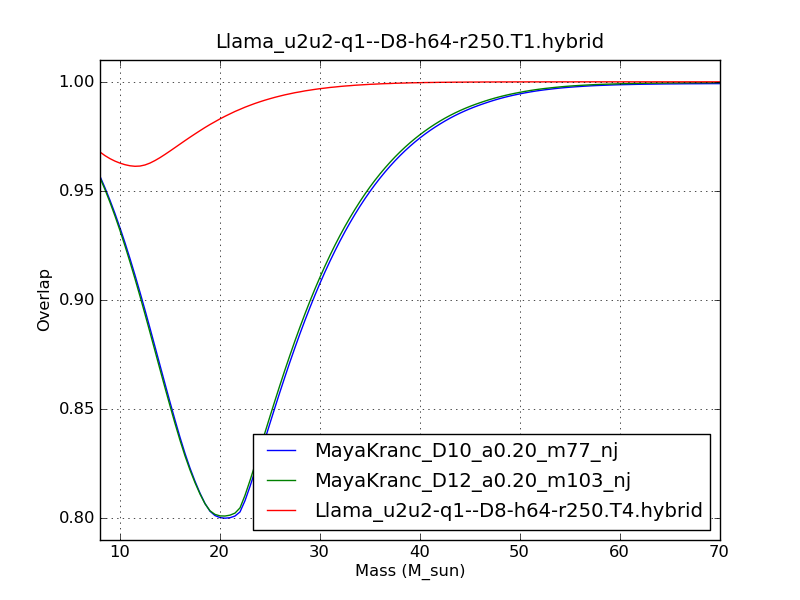
\includegraphics[width=0.5\linewidth]{figures/ninja2/figure_1_0d2_09.png} 
  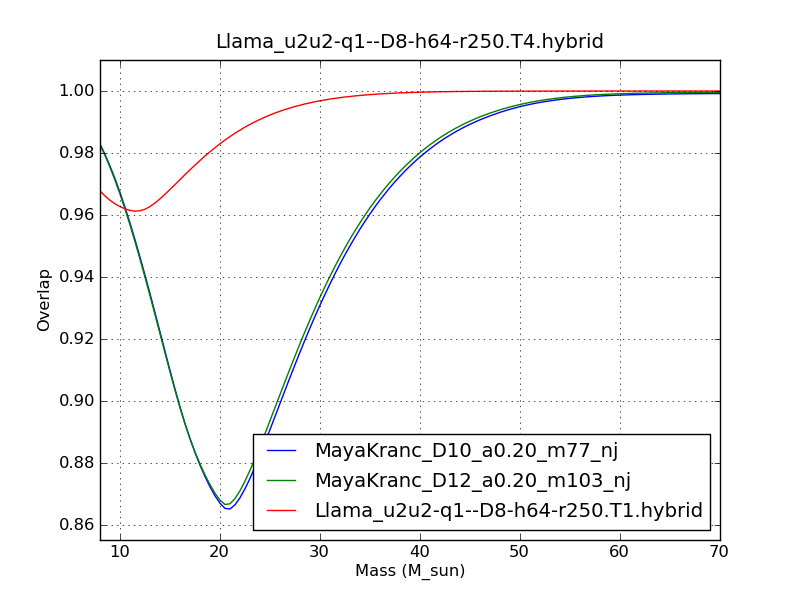
\includegraphics[width=0.5\linewidth]{figures/ninja2/figure_1_0d2_12.png} \\
  \caption[Overlap plots for $q=1$ $S_{z1} = S_{z2} = 0.2$]{
  \label{f:figure_1_0d2}
Overlap plots for $q=1$ $S_{z1} = S_{z2} = 0.2$}
\end{figure}%


\begin{figure}
  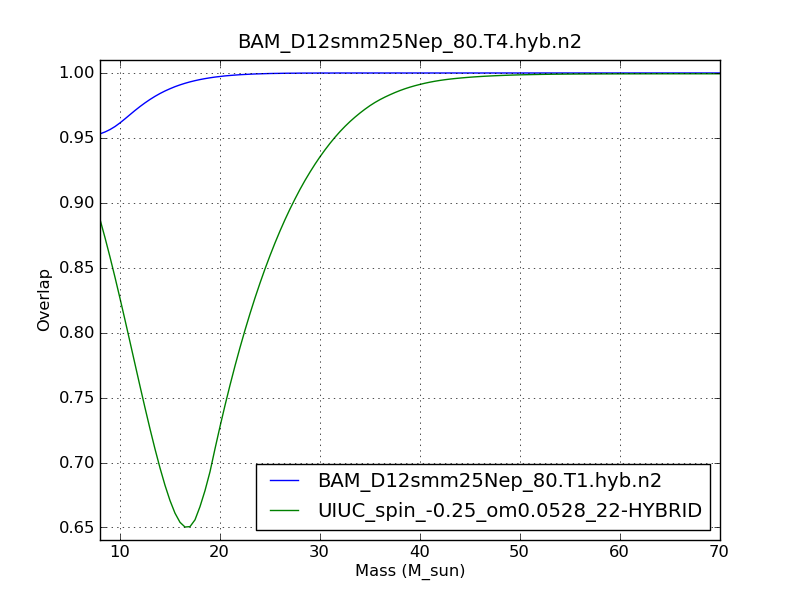
\includegraphics[width=0.5\linewidth]{figures/ninja2/figure_1_-0d25_02.png} 
  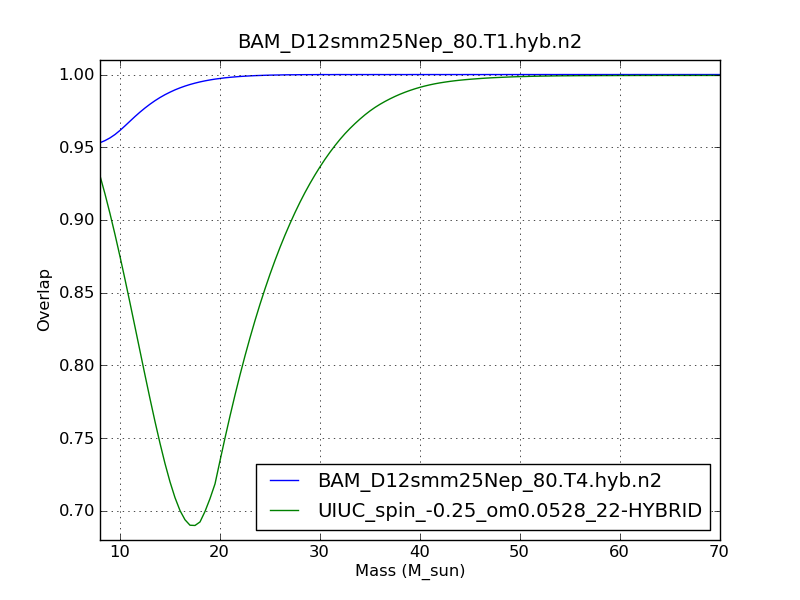
\includegraphics[width=0.5\linewidth]{figures/ninja2/figure_1_-0d25_04.png} \\
  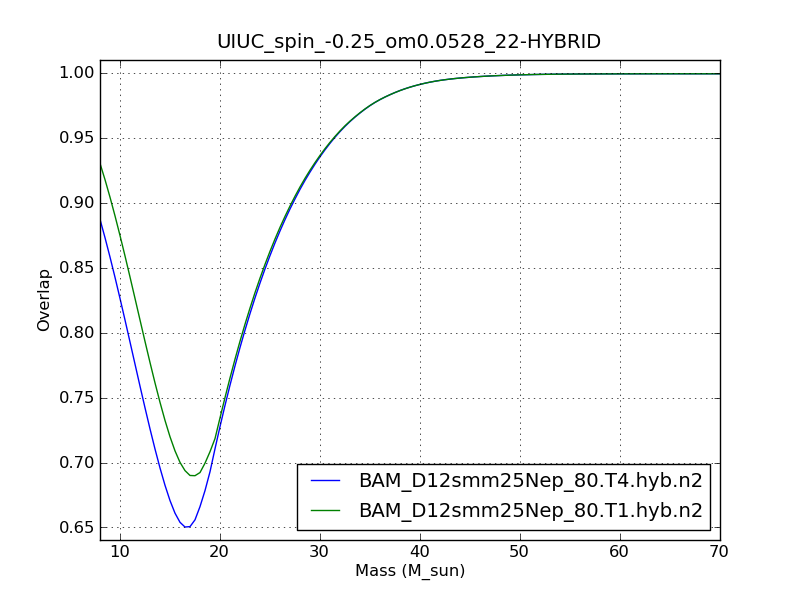
\includegraphics[width=0.5\linewidth]{figures/ninja2/figure_1_-0d25_06.png} 
  \caption[Overlap plots for $q=1$ $S_{z1} = S_{z2} = -0.25$]{
  \label{f:figure_1_-0d25}
Overlap plots for $q=1$ $S_{z1} = S_{z2} = -0.25$}
\end{figure}%


\begin{figure}
  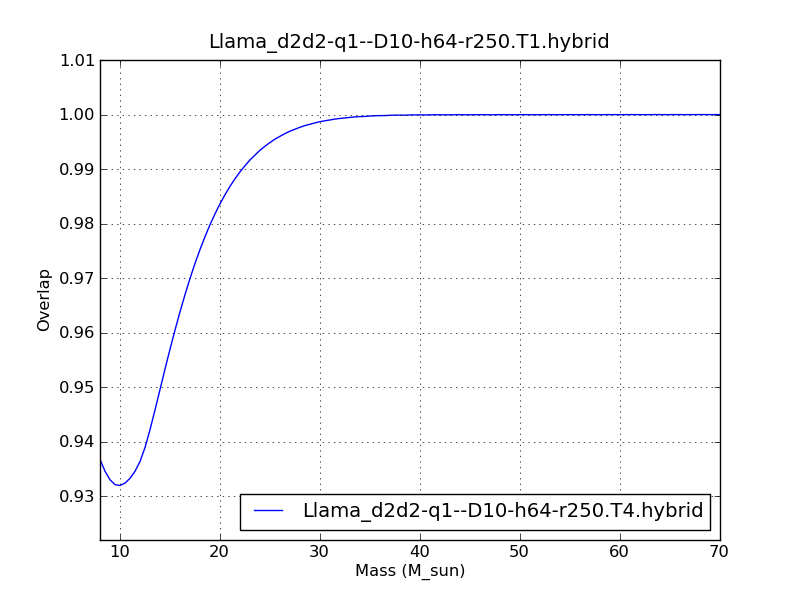
\includegraphics[width=\linewidth]{figures/ninja2/figure_1_-0d2_01.png}
  \caption[Overlap plots for $q=1$ $S_{z1} = S_{z2} = -0.2$]{
  \label{f:figure_1_-0d2}
Overlap plots for $q=1$ $S_{z1} = S_{z2} = -0.2$}
\end{figure}%


\begin{figure}
  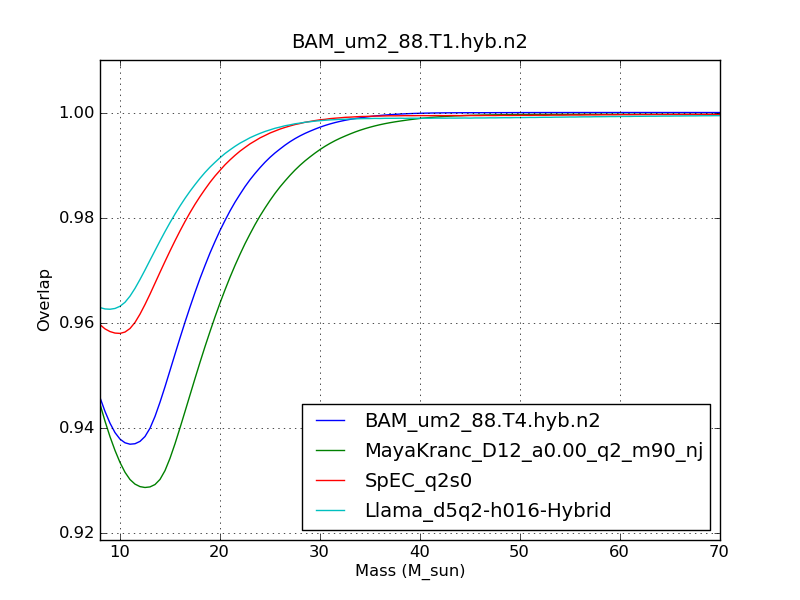
\includegraphics[width=0.5\linewidth]{figures/ninja2/figure_2_0_04.png} 
  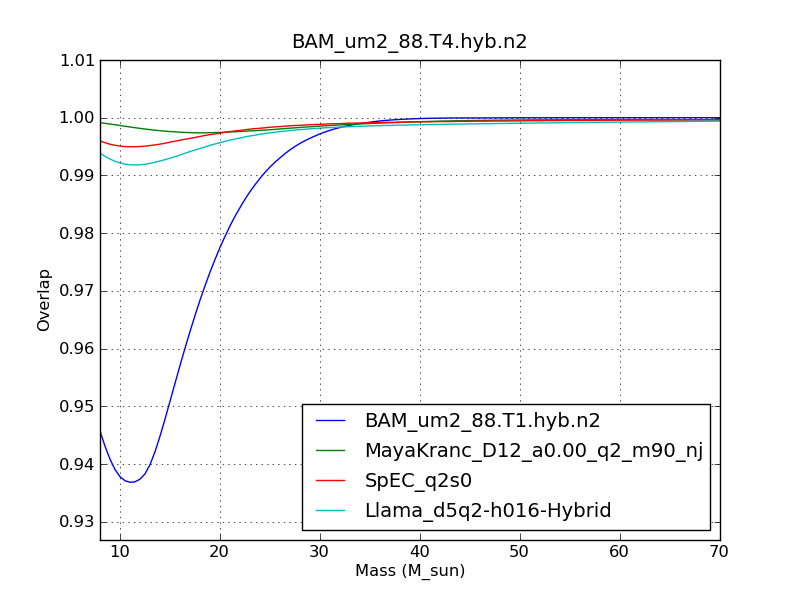
\includegraphics[width=0.5\linewidth]{figures/ninja2/figure_2_0_08.png} \\
  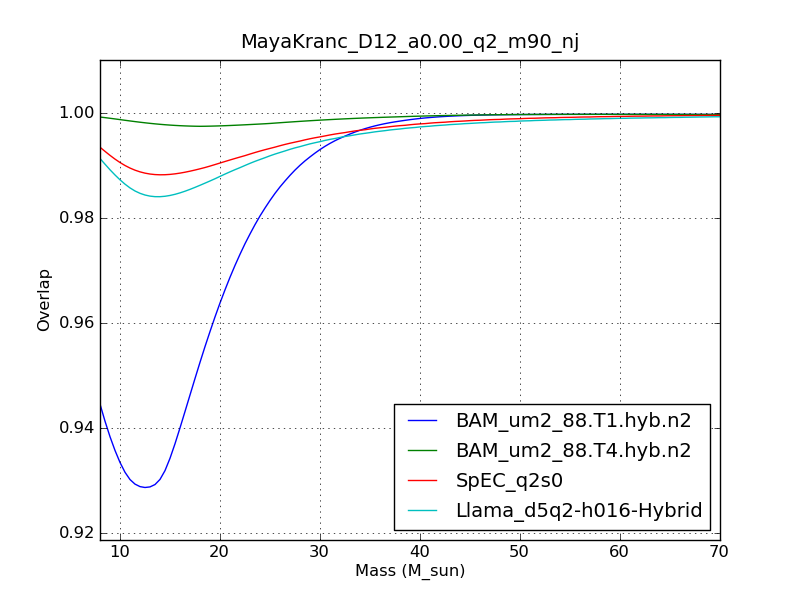
\includegraphics[width=0.5\linewidth]{figures/ninja2/figure_2_0_12.png} 
  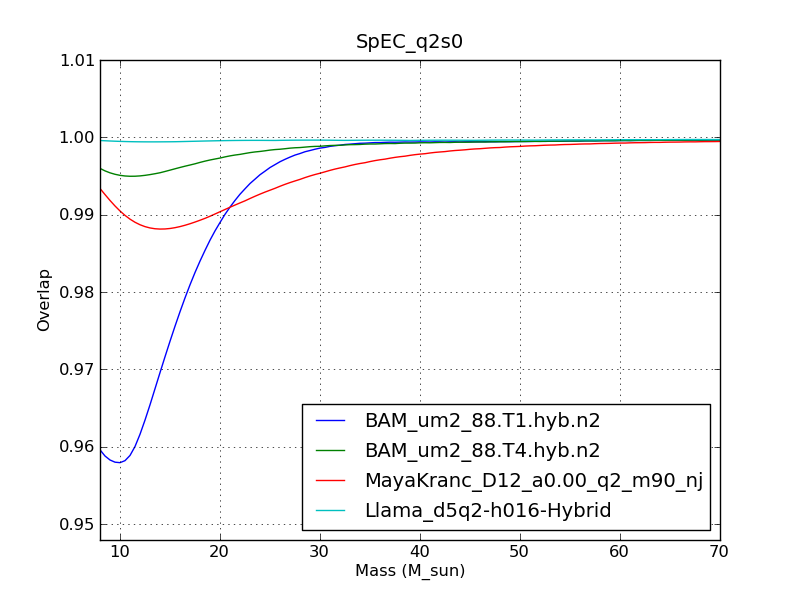
\includegraphics[width=0.5\linewidth]{figures/ninja2/figure_2_0_16.png} \\
  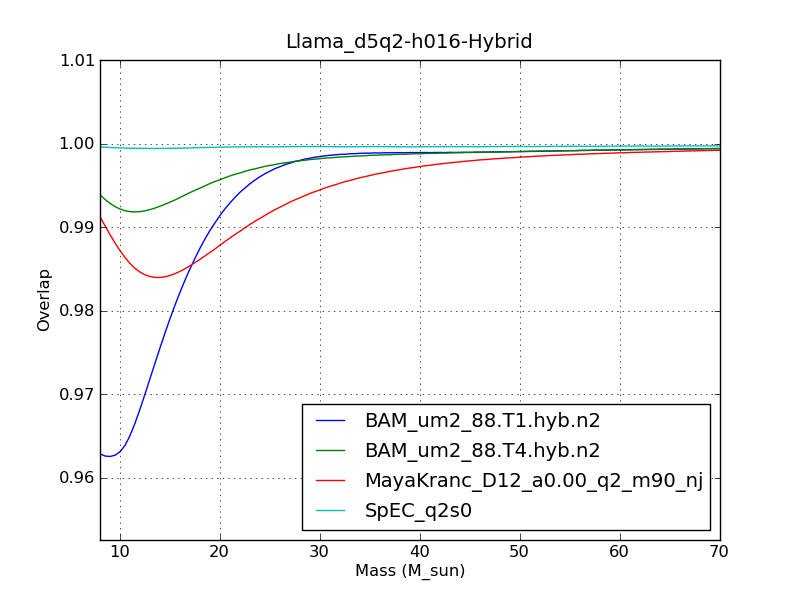
\includegraphics[width=0.5\linewidth]{figures/ninja2/figure_2_0_20.png} 
  \caption[Overlap plots for $q=2$ $S_{z1} = S_{z2} = 0$]{
  \label{f:figure_2_0}
Overlap plots for $q=2$ $S_{z1} = S_{z2} = 0$}
\end{figure}%


\begin{figure}
  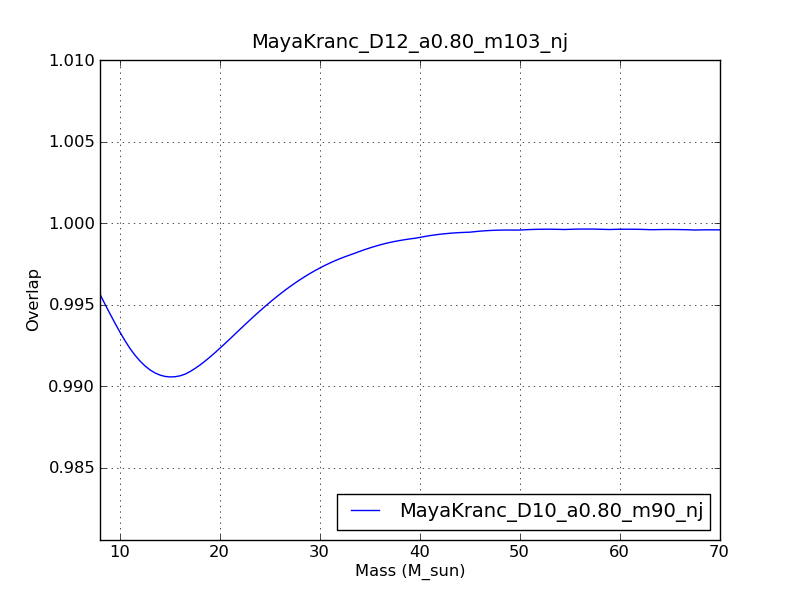
\includegraphics[width=\linewidth]{figures/ninja2/figure_1_0d8_01.png}
  \caption[Overlap plots for $q=1$ $S_{z1} = S_{z2} = 0.8$]{
  \label{f:figure_1_0d8}
Overlap plots for $q=1$ $S_{z1} = S_{z2} = 0.8$}
\end{figure}%


\begin{figure}
  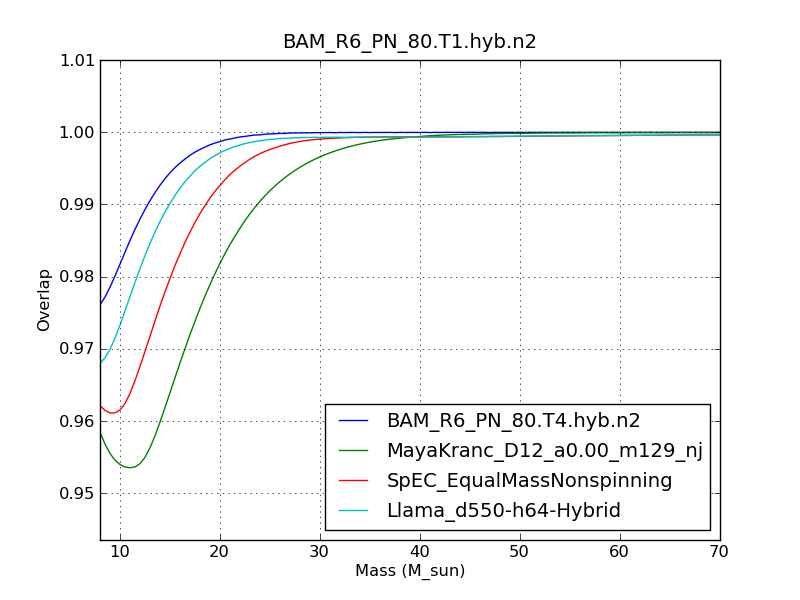
\includegraphics[width=0.5\linewidth]{figures/ninja2/figure_1_0_04.png} 
  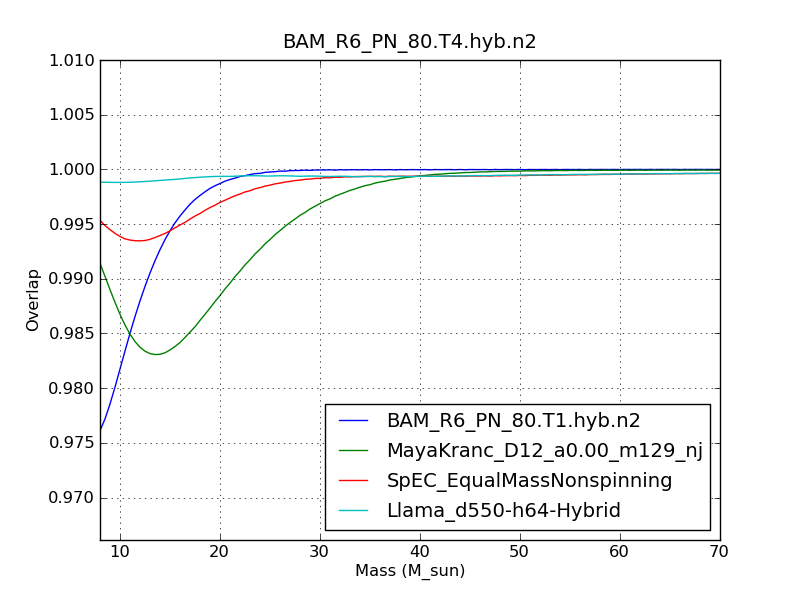
\includegraphics[width=0.5\linewidth]{figures/ninja2/figure_1_0_08.png} \\
  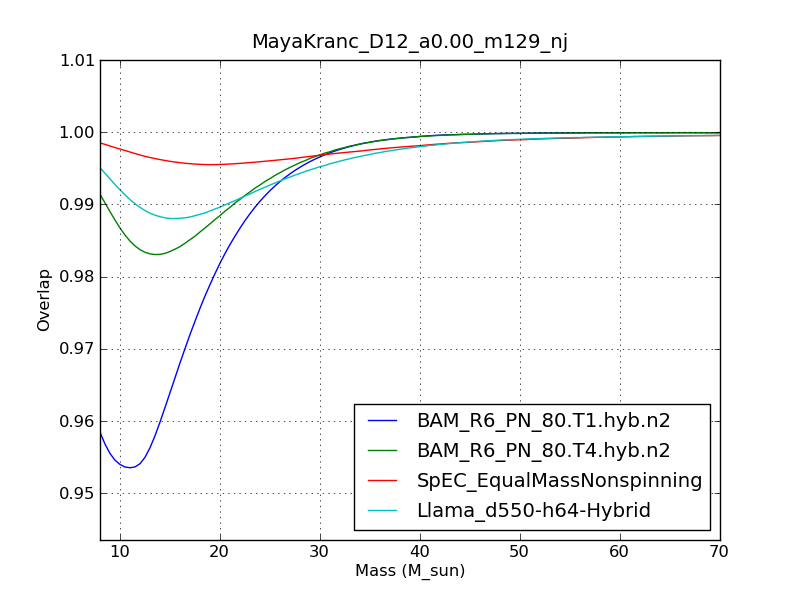
\includegraphics[width=0.5\linewidth]{figures/ninja2/figure_1_0_12.png} 
  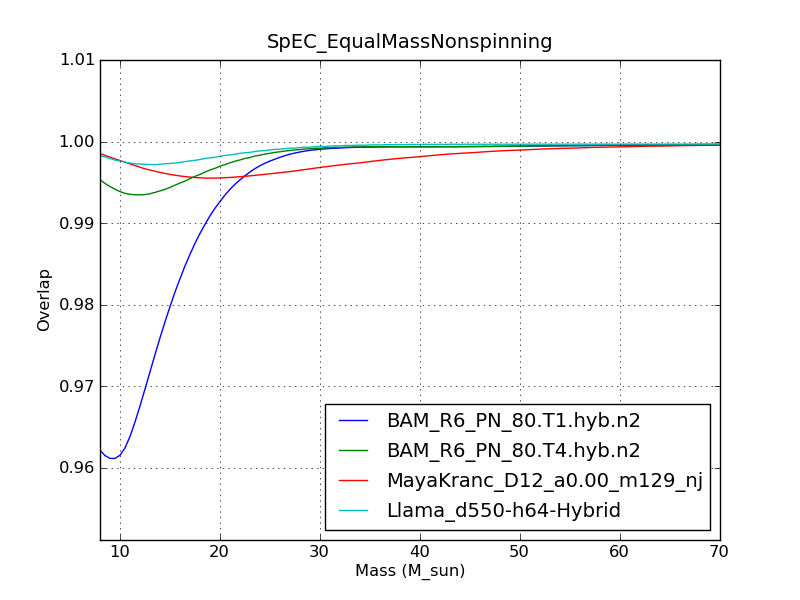
\includegraphics[width=0.5\linewidth]{figures/ninja2/figure_1_0_16.png} \\
  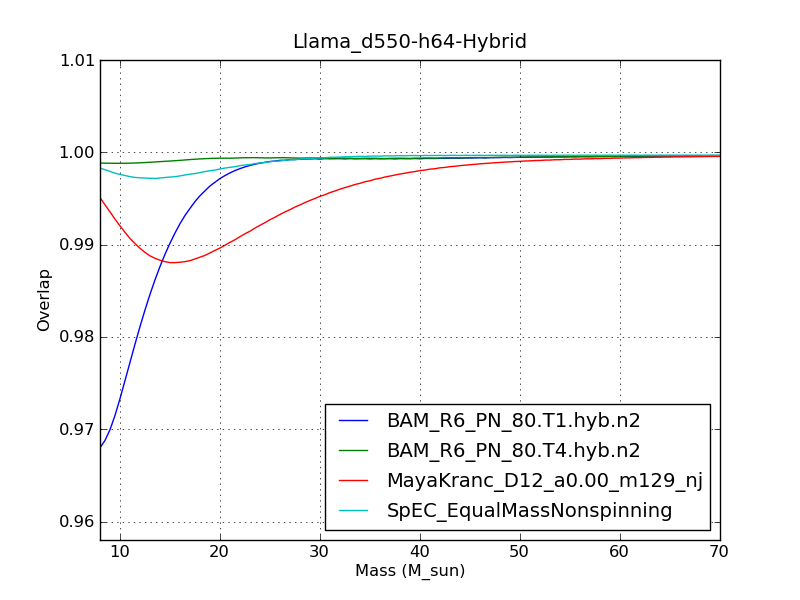
\includegraphics[width=0.5\linewidth]{figures/ninja2/figure_1_0_20.png} 
  \caption[Overlap plots for $q=1$ $S_{z1} = S_{z2} = 0$]{
  \label{f:figure_1_0}
Overlap plots for $q=1$ $S_{z1} = S_{z2} = 0$}
\end{figure}%


\begin{figure}
  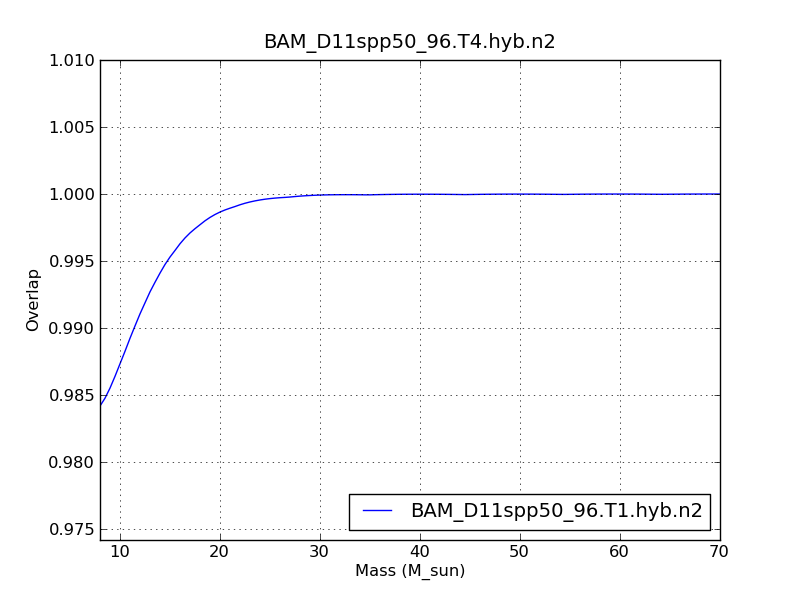
\includegraphics[width=\linewidth]{figures/ninja2/figure_1_0d5_01.png}
  \caption[Overlap plots for $q=1$ $S_{z1} = S_{z2} = 0.5$]{
  \label{f:figure_1_0d5}
Overlap plots for $q=1$ $S_{z1} = S_{z2} = 0.5$}
\end{figure}%


\begin{figure}
  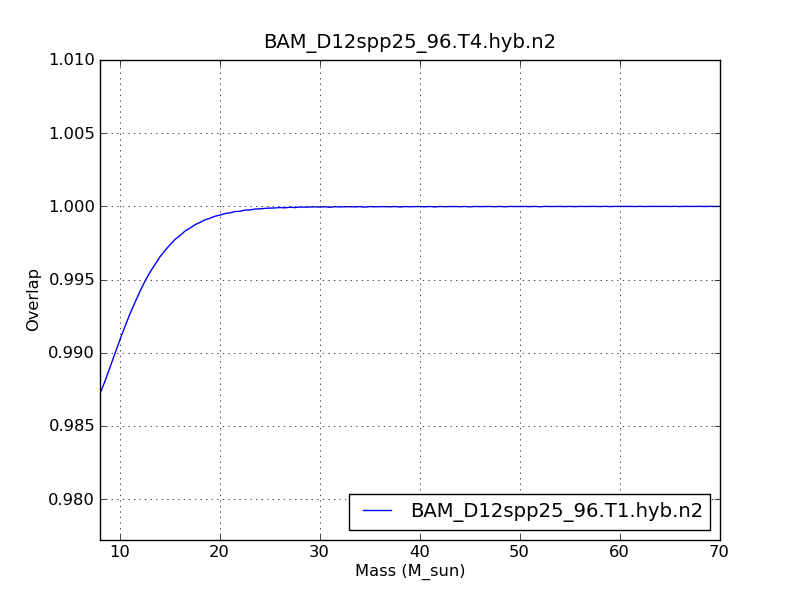
\includegraphics[width=\linewidth]{figures/ninja2/figure_1_0d25_01.png}
  \caption[Overlap plots for $q=1$ $S_{z1} = S_{z2} = 0.25$]{
  \label{f:figure_1_0d25}
Overlap plots for $q=1$ $S_{z1} = S_{z2} = 0.25$}
\end{figure}%


\begin{figure}
  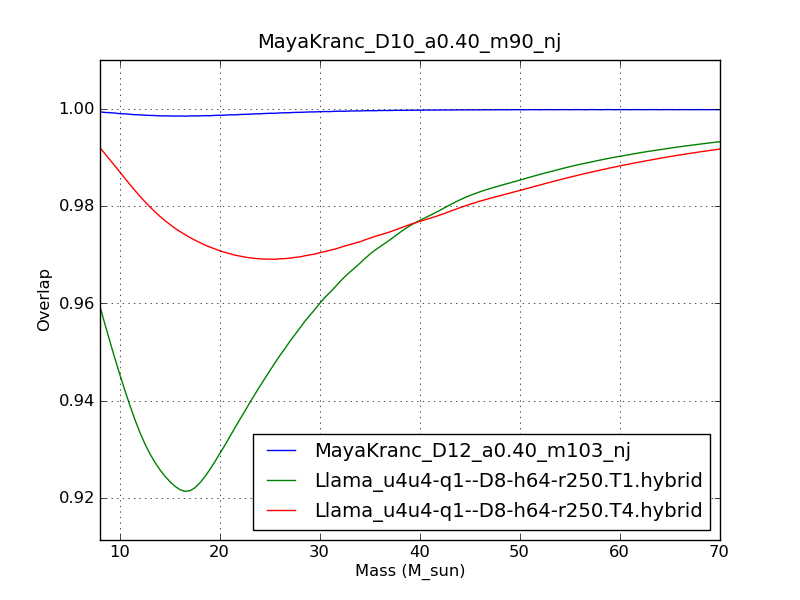
\includegraphics[width=0.5\linewidth]{figures/ninja2/figure_1_0d4_03.png} 
  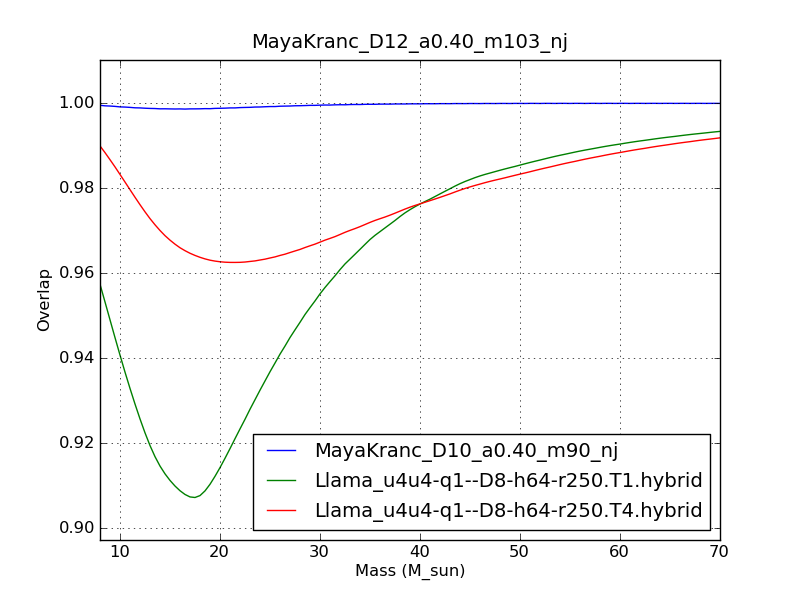
\includegraphics[width=0.5\linewidth]{figures/ninja2/figure_1_0d4_06.png} \\
  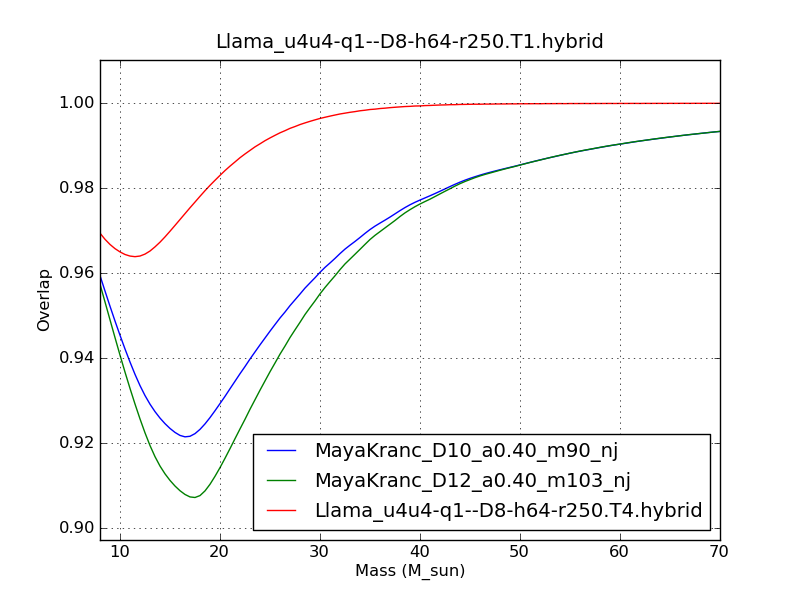
\includegraphics[width=0.5\linewidth]{figures/ninja2/figure_1_0d4_09.png} 
  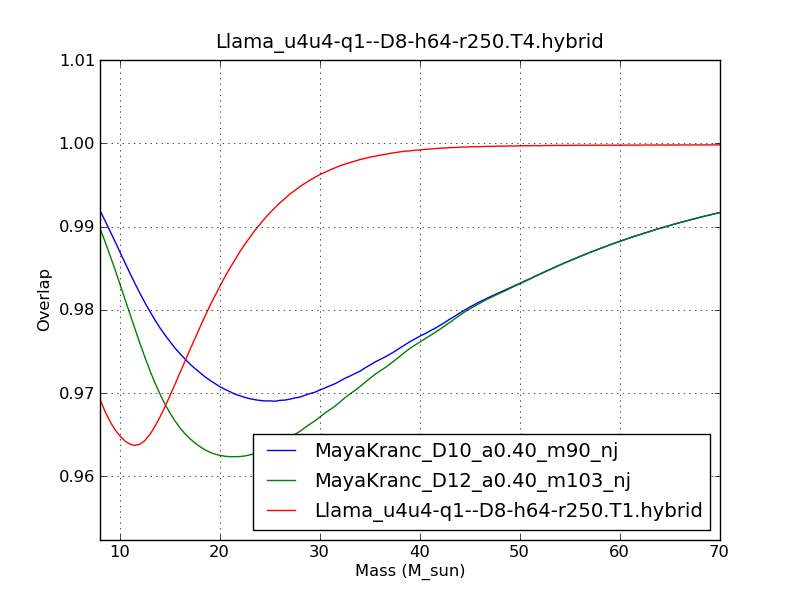
\includegraphics[width=0.5\linewidth]{figures/ninja2/figure_1_0d4_12.png} \\
  \caption[Overlap plots for $q=1$ $S_{z1} = S_{z2} = 0.4$]{
  \label{f:figure_1_0d4}
Overlap plots for $q=1$ $S_{z1} = S_{z2} = 0.4$}
\end{figure}%


\begin{figure}
  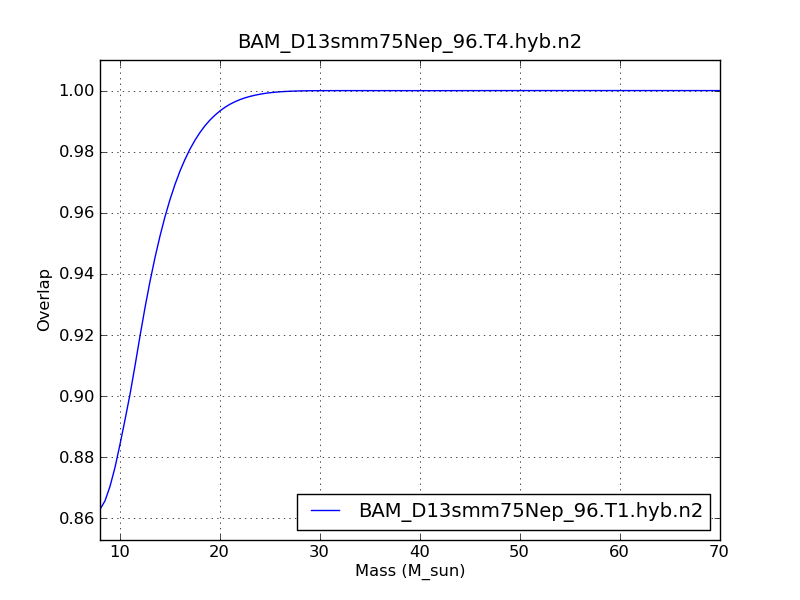
\includegraphics[width=\linewidth]{figures/ninja2/figure_1_-0d75_01.png}
  \caption[Overlap plots for $q=1$ $S_{z1} = S_{z2} = -0.75$]{
  \label{f:figure_1_-0d75}
Overlap plots for $q=1$ $S_{z1} = S_{z2} = -0.75$}
\end{figure}%


\begin{figure}
  \includegraphics[width=\linewidth]{figures/ninja2/figure_1_-0d85_01.png}
  \caption[Overlap plots for $q=1$ $S_{z1} = S_{z2} = -0.85$]{
  \label{f:figure_1_-0d85}
Overlap plots for $q=1$ $S_{z1} = S_{z2} = -0.85$}
\end{figure}%


\begin{figure}
  \includegraphics[width=0.5\linewidth]{figures/ninja2/figure_4_0_03.png} 
  \includegraphics[width=0.5\linewidth]{figures/ninja2/figure_4_0_06.png} \\
  \includegraphics[width=0.5\linewidth]{figures/ninja2/figure_4_0_09.png} 
  \includegraphics[width=0.5\linewidth]{figures/ninja2/figure_4_0_12.png} \\
  \caption[Overlap plots for $q=4$ $S_{z1} = S_{z2} = 0$]{
  \label{f:figure_4_0}
Overlap plots for $q=4$ $S_{z1} = S_{z2} = 0$}
\end{figure}%


\begin{figure}
  \includegraphics[width=\linewidth]{figures/ninja2/figure_1_0d75_01.png}
  \caption[Overlap plots for $q=1$ $S_{z1} = S_{z2} = 0.75$]{
  \label{f:figure_1_0d75}
Overlap plots for $q=1$ $S_{z1} = S_{z2} = 0.75$}
\end{figure}%


\begin{figure}
  \includegraphics[width=0.5\linewidth]{figures/ninja2/figure_1_0d85_02.png} 
  \includegraphics[width=0.5\linewidth]{figures/ninja2/figure_1_0d85_04.png} \\
  \includegraphics[width=0.5\linewidth]{figures/ninja2/figure_1_0d85_06.png} 
  \caption[Overlap plots for $q=1$ $S_{z1} = S_{z2} = 0.85$]{
  \label{f:figure_1_0d85}
Overlap plots for $q=1$ $S_{z1} = S_{z2} = 0.85$}
\end{figure}%

\clearpage
%%%%%%%%%%%%%%%%

